\documentclass{article}
\usepackage{graphicx}
\usepackage{amsmath}
\PassOptionsToPackage{svgnames}{xcolor}
\usepackage{tcolorbox}
\usepackage{xcolor}
\usepackage{lipsum}
\usepackage{verbatim}
\tcbuselibrary{skins,breakable}
\usetikzlibrary{shadings,shadows}
\usepackage{float}
\usepackage{hyperref}
\usepackage[a4paper]{geometry}
\usepackage{listings}
\usepackage{titlesec}
\usepackage{amssymb}
\usepackage[T1]{fontenc}
\usepackage{multirow} % for Tables
\usepackage{fancyvrb} % for "\Verb" macro
\VerbatimFootnotes % enable use of \Verb in footnotes
\usepackage{listings}
\lstset{basicstyle=\ttfamily,
  showstringspaces=false,
  commentstyle=\color{green},
  keywordstyle=\color{blue}
}

\setcounter{secnumdepth}{4}
\titleformat{\paragraph}
{\normalfont\normalsize\bfseries}{\theparagraph}{1em}{}
\titlespacing*{\paragraph}
{0pt}{3.25ex plus 1ex minus .2ex}{1.5ex plus .2ex}

\title{\textbf{Terraform}}
\author{Alejandro Campos}
\date{June, 2024}

\setlength{\parindent}{0ex}
\setlength{\parskip}{6pt}
\geometry{top=2.5cm, bottom=3cm,left=3cm, right=3cm}
\hypersetup{
    colorlinks=true,
    linkcolor=black,
    filecolor=magenta,
    urlcolor=blue,
}

\definecolor{codegreen}{rgb}{0,0.6,0}
\definecolor{codegray}{rgb}{0.5,0.5,0.5}
\definecolor{codepurple}{rgb}{0.58,0,0.82}
\definecolor{backcolour}{rgb}{0.95,0.95,0.92}

\newenvironment{blocktemplate}[1]{%
    \tcolorbox[beamer,%
    noparskip,breakable,
    colframe=Blue,%
    colbacklower=LimeGreen!75!LightGreen,%
    title=#1]}%
    {\endtcolorbox}

\newenvironment{blocktemplateI}[1]{%
    \tcolorbox[beamer,%
    noparskip,breakable,
    colframe=Violet,%
    colbacklower=Black,%
    title=#1]}%
    {\endtcolorbox}

\newenvironment{blocktemplateII}[1]{%
    \tcolorbox[beamer,%
    noparskip,breakable,
    colframe=Green,%
    colbacklower=LimeGreen!75!LightGreen,%
    title=#1]}%
    {\endtcolorbox}

\newenvironment{blocktemplateIII}[1]{%
    \tcolorbox[beamer,%
    noparskip,breakable,
    ,colframe=Red,%
    colbacklower=LimeGreen!75!LightGreen,%
    title=#1]}%
    {\endtcolorbox}

\newtcolorbox{mybasecolorbox}[1][]{%
  colback=gray!25, colframe=gray!25,
  coltitle=black,
  width=(\linewidth-20pt)}

\newenvironment{codetemplate}[1][]{%
  \mybasecolorbox[#1]
  \itshape
}{%
  \endmybasecolorbox
}

\begin{document}
\maketitle
\newpage
\tableofcontents

%====================================================================================================
\newpage
\section{Introduction}
\subsection{Necessity of Terraform}
In the traditional IT model, infrastructure is provisioned as following (aprox.):
\begin{enumerate}
    \item Bussiness comes up with the requirements for the new application.
    \item Bussines analysts conver them into a set of high-lvl technical requirements.
    \item Solution Architects designs the architecture to be followed for the deployment of this application, considering Front-End, Back-End, Databases, Load Balancers, etc.:
    \begin{itemize}
        \item Number of servers needed.
        \item Specifications of these servers.
        \item Type of servers.
    \end{itemize}
    \item Once it is planned, it should be deployed on the Onpremise servers from the organization.
    \item If additional harwar is needed, they would have to be ordered, which can take few days, weeks or even months for the hardware to be purchased and delivered to the datacenter.
    \item Once the hardware is on the datacenter, Infrastructure Engineers will rack and stack all the equipment.
    \item The System Administrators will perform initial configurations on all the servers.
    \item The Network Adminisrtators will configure and wire all the equipment to connect them to the organization network.
    \item The Storage Admin assign the storage to the servers and configure backups.
    \item Then, the application is ready for the developer teams in order to deploy their applications.
\end{enumerate}

This procedure has some disadvantages:
\begin{enumerate}
    \item The whole process can take between few weeks to few months, and it is just to have the hardware in a ready state to begin the application deployment.
    \item Saling up / scaling down the infrastructure on demand it is costly and time-consuming.
    \item \textbf{Underutilization of compute resources:} the servers are usualy virtualized, and the VM's are always sized considering the peak utilization. So the inability to scale up or down easily means that most of these resources wouldn't be used during tha vast majority of the time (off-peak hours).
\end{enumerate}

And they are some of the reasons why organizations have been moving  to virtualization and cloud platforms, such as: Amazon AWS, Azure, IBM Cloud, Google Cloud, etc. By moving to cloud, the time to spin up the infrastructure when Bussiness comes up with the requirements for the new application is significantly reduced. So the time to market is significantly reduced as well.

Furthermore, another advantage on Cloud, is that organizations do not have to invest in or manage the hardware assets as in a traditional infrastructure model. The datacenter, the hardware assets and the services are managed by the cloud provider.

A VM can be provisioned in a matter of minutes in a Cloud Environment, and the time to market can be reduced in several months. Besides, infrastructure costs are reduced due to the no need of a datacenter neither human resources to manage it. Furthermore, it is easily scalable and reduce the underutilization of compute resources.

Cloud Infrastrucute come with API's and that opens a whole new world of opportunity for automation. As well as GUI where VM's can be provisioned with a few clicks (and a cash flow). But, when you have to handle with large infrastructure, manage it manually through the GUI's is not the ideal. That's when \textbf{Terraform} come in place, a tool for automate infrastructure provisioning to deploy environments faster in a consistent fashion using the different API's from the various cloud providers.

\subsection{Infrastructure as Code (IaC)}
The better way to provision cloud environment resources is codifying the entire provisioning process, this way we can write, execute and store code to: define, provision, configure, update, upgrade and destroy infrastructure resources. With IaC, any infrastructure component can be managed as code, such as: server, databases, networks, storage, app configurations. Tools like Ansible, Docker, Vagran, Puppet, Terraform are IaC examples, which are easy to learn languages to easily manage infrastructure.

With IaC we can define infrastructure resources using simple, human readable, high-level language. They can be categorized into 3 types:

\begin{itemize}
    \item \textbf{Infrastructure Configuration Management:} used to install and manage existing infrastructure resources, such as: server, databases, networking devices, etc. They are designed to run into multiple instances at once but they best feature is that they are \textbf{idemportent}; so the same code can be run multiple times and the result will be the same, making just the necessary changes and not more. Examples:
    \begin{itemize}
        \item Ansible
        \item Puppet
    \end{itemize}
    \item \textbf{Server Templating:} used to create custom static images from VM's or containers, containing all the required software and dependencies. They promote immutable infrastructure, unlike Infrastructure Configuration Management tools, so once the VM or the contaner is deployed, it is designed to remain unchanged (static). In case of changes to be made on the images, instead of updating the running instance, update on the image is needed and then re-deploy a new instance into a container.
    \begin{itemize}
        \item Docker
        \item Podman
        \item Vagrant
        \item Packer
    \end{itemize}
    \item \textbf{Infrastructure Provisioning Tools:} used to provision infrastructure components using simple and declarative code, such as: servers, VM's, databases, VPC's (Private Cloud Network), subnets, security groups, storage, etc. They use to be \textbf{provider agnostic} (Terraform is), which means that they are compatible with almost all major cloud providers, having their plugins.
    \begin{itemize}
        \item Terraform
    \end{itemize}
\end{itemize}

\subsection{Why Terraform?}
Terraform is one of the most populars IaC tools, beloging Infrastructure Provisioning type, open-source developer by HasiCorp. It is installed as a single binary which can be set up quickly allowing us to create, update, upgrade, destroy, configure and manage infrastructure in a matter of minutes. It is \textbf{provider agnostic}, so it can deploy infrastructure across multiple platforms, includin gprivate and public clouds.

Terraform can deploy in so many different cloud thanks to \textbf{provides}, they help Terraform to manage third-party plaftorms thourgh their API.

\begin{itemize}
    \item Onpremise
    \item VMWare Machines
    \item AWS
    \item Google Cloud
    \item Azure
    \item ...
\end{itemize}

Terraform uses HCL (Hashicorp Configuration Language - .tf extension), which is a simple declarative language to define the infrastructure resources to be provisioned as blocks of code. Terraform will take care of what is required to go from the current state of the infrastructure to the desired state (the one defined on the HLC files).

Every object that Terraform manages is called a resource, which can be a compute instace, a server, a VM, a database, etc. Terraform will mage the lifecycle of the resource from its provisioning, to configuration, to decommissioning. It can ensure that the entire infrastructure is always in the defined state at all times.

\begin{figure}[H]
    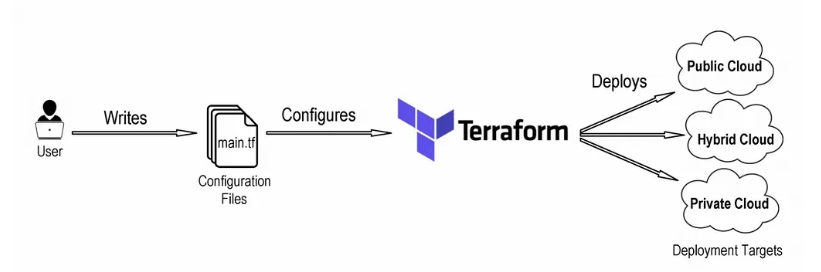
\includegraphics[width=\textwidth]{pictures/pic1.png}
    \centering
\end{figure}

%====================================================================================================
\newpage
\section{Terraform Basics}

\subsection{Installing Terraform}

\begin{enumerate}
    \item Update the package list
\begin{codetemplate}{}
\begin{verbatim}
$ sudo apt-get update
\end{verbatim}
\end{codetemplate}

    \item Add the HashiCorp GPG key:
\begin{codetemplate}{}
\begin{verbatim}
$ curl -fsSL https://apt.releases.hashicorp.com/gpg \ 
| sudo apt-key add -
\end{verbatim}
\end{codetemplate}

    \item Add the official HashiCorp Linux repository:
\begin{codetemplate}{}
\begin{verbatim}
$ sudo apt-add-repository \
"deb [arch=amd64] https://apt.releases.hashicorp.com \
$(lsb_release -cs) main"
\end{verbatim}
\end{codetemplate}

    
    \item Update the package list again:
\begin{codetemplate}{}
\begin{verbatim}
$ sudo apt-get update
\end{verbatim}
\end{codetemplate}

    \item Install Terraform:
\begin{codetemplate}{}
\begin{verbatim}
$ sudo apt-get install -y terraform
\end{verbatim}
\end{codetemplate}

    \item Check terraform is installed
\begin{codetemplate}{}
\begin{verbatim}
$ terraform verion
\end{verbatim}
\end{codetemplate}
\end{enumerate}

\subsection{My first Terraform Provision}

\subsubsection{HCL (.tf - HashiCorp Configuration Language)}
The HCL files contains block and arguments:
\begin{itemize}
    \item \textbf{Blocks:} they contains information about the infrastructure platform and a set of resrouces within that platform that we want to create.
    \item \textbf{Arguments:} the configuration of them (inside \verb|{}|), they are specific to the type of resource we are creating.
\end{itemize}

\begin{codetemplate}{}
\begin{verbatim}
<block> <parameters> {
    key1 = value1
    key2 = value2
}
\end{verbatim}
\end{codetemplate}

For example, imagine that we want to create a file in local host:
\begin{codetemplate}{local.tf}
\begin{verbatim}
resource "local_file" "cats" {
    filename = "/tmp/cats.txt"
    content  = "I love cats!"
}
\end{verbatim}
\end{codetemplate}

\begin{itemize}
    \item \textbf{Block Name:} resource
    \item \textbf{Resource Type:} \verb+local_file+ 
    \begin{itemize}
        \item \textbf{Provider:} local
        \item \textbf{Resource Type:} file
    \end{itemize}
    \item \textbf{Resource Name:} cats
    \item \textbf{Arguments:}
    \begin{itemize}
        \item \textbf{filename:} "/tmp/cats.txt"
        \item \textbf{content:} "I love cats!"
    \end{itemize}
\end{itemize}

As another example here we have an HCL file to create an AWS S3 bucket:
\begin{codetemplate}{aws-s3.tf}
\begin{verbatim}
resource "aws_s3_bucket" "data-bucket" {
    bucket  = "webserver-bucket-org-2207"
    content = "private"
}
\end{verbatim}
\end{codetemplate}

\subsubsection{Terraform WorkFlow}
The simple Terraform workflow consists of 4 steps:

\begin{enumerate}
    \item Write the HCL (.tf) configuration files
    \item Run the \textbf{terraform init} command, which will check the configuration files and initialize the working directory containing the .tf file.
\begin{codetemplate}{}
\begin{verbatim}
$ terraform init
\end{verbatim}
\end{codetemplate}
    \item Review the execution plan using \textbf{terraform plan} command, to see the execution plan that will be carried out by Terraform, which will show the actions that will be carried out by Terraform to create the resources, like:
\begin{itemize}
    \item \verb+diff+ command in \verb+git+
    \item \verb+--checkout --diff+ in \verb+Ansible+
\end{itemize} 
\begin{codetemplate}{This won't apply anything, just check}
\begin{verbatim}
$ terraform plan
\end{verbatim}
\end{codetemplate}
    \item Apply the changes using the \textbf{terraform apply} command, which will display the execution plan once again and it will ask to confirm by typing \verb+Yes+ to proceed. Once we confirm, it will proceed with the creation, update, deletion of the resources
\begin{codetemplate}{}
\begin{verbatim}
$ terraform apply
\end{verbatim}
\end{codetemplate}
\end{enumerate}

\begin{blocktemplateI}{Note}
Terraform show command can also be run to see the deatils of the resources that we just created
\end{blocktemplateI}

\begin{figure}[H]
    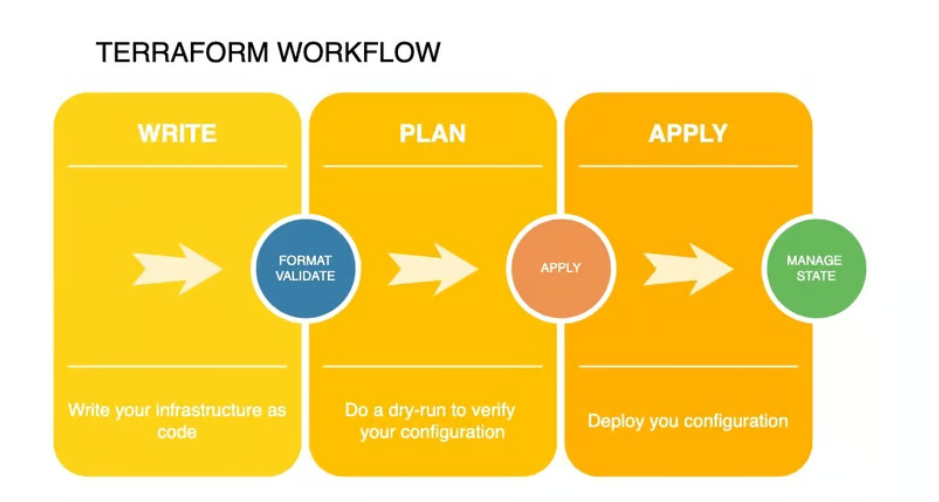
\includegraphics[width=\textwidth]{pictures/pic2.png}
    \centering
\end{figure}

\subsubsection{Provider, Resource Types and their custom Arguments}
How can we know the availabe resources types from a terraform provider, and how can we know the arguments we can use on this resource type? Terraform has hundreds of providers (they are like modules in Ansible), including the \verb+local_provider+ we have used in the example. Each provider has a unique list of resource types that can be created on that specific platform, and each resource type can have different (required or optional) arguments to create the resource.

Examples of other providers:

\begin{itemize}
    \item \href{https://registry.terraform.io/providers/hashicorp/local/latest}{local}:  used to manage local resources, such as files.
    \item \href{https://registry.terraform.io/providers/hashicorp/aws/latest}{aws}: provider used to lifecycle management of AWS resources, including EC2, Lambda, EKS, ECS, VPC, S3, RDS, DynamoDB, and more. This provider is maintained internally by the HashiCorp AWS Provider team.
    \item \href{https://registry.terraform.io/providers/hashicorp/azurerm/latest}{azurerm}: provider used to lifecycle management of Microsoft Azure using the Azure Resource Manager APIs. maintained by the Azure team at Microsoft and the Terraform team at HashiCorp.
    \item \href{https://registry.terraform.io/providers/hashicorp/google/latest}{google}: provider used to lifecycle management of GCP resources, including Compute Engine, Cloud Storage, Cloud SDK, Cloud SQL, GKE, BigQuery, Cloud Functions and more. This provider is collaboratively maintained by the Google Terraform Team at Google and the Terraform team at HashiCorp.
    \item \href{https://registry.terraform.io/providers/hashicorp/helm/latest}{helm}: provider used to deploy software packages in Kubernetes using Helm.
    \item \href{https://registry.terraform.io/providers/hashicorp/kubernetes/latest}{kubernetes}: provider used to manage of all Kubernetes resources, including Deployments, Services, Custom Resources (CRs and CRDs), Policies, Quotas and more.
    \item \href{https://registry.terraform.io/providers/aliyun/alicloud/latest}{alicloud}: provider used to interact with the many resources supported by Alibaba Cloud. The provider needs to be configured with the proper credentials before it can be used.
    \item ...
\end{itemize}

To know all the available providers, check the \href{https://registry.terraform.io/browse/providers}{Official Terraform Registry Providers}

\subsection{Update and Destroy Infrastructure}

Taking the previous example of the file, let's see how can we update and destroy this resources. 

\subsubsection{Update}
For update is very easy, we just need to modify the field we want and then run again the 2 last steps:
\begin{codetemplate}{}
\begin{verbatim}
$ terraform plan
\end{verbatim}
\end{codetemplate}

Even though the update is trivial, as \textbf{file resource type} is \textbf{immutable infrastructure} Terraform will \textbf{always delete the old resource and then create a new resource} when updating an \textbf{immutable resource}. So taking this into account, if you are agree with the changes:
\begin{codetemplate}{}
\begin{verbatim}
$ terraform apply
\end{verbatim}
\end{codetemplate}

\subsubsection{Delete}
To remove completely the resources within a configuration directory, run:
\begin{codetemplate}{}
\begin{verbatim}
$ terraform destroy
\end{verbatim}
\end{codetemplate}

You will be asked to confirm the destroy, so type \verb+yes+ in the prompt and it will delete all the resources in the current configuration directory.


\subsection{More details on Terraform Providers}
The first action Terraform does when we run \verb|terraform init| within a directory containing the configuration files, it downloads and installs all the plugins needed to provision the resources defined on the repository. Terraform providers are distributed by HashiCorp and they are open-source available at \href{https://registry.terraform.io/}{Terraform Registry}.

There are 3 tiers of providers:

\begin{itemize}
    \item \textbf{Official Providers:} owned and mantained by HashiCorp, and include the major cloud providers such as AWS, GCP, Azure, etc.
    \item \textbf{Partner Providers:} owned and mantianed by a third-party technology company that has gone through a partner provider process with HashiCorp.
    \item \textbf{Community Providers:} published, owned and mantainer by individual contributors of the HashiCorp community.
\end{itemize}

The \verb+terraform init+ command, shows the version of the plugins it is installing, and then it downloads and store them into the hidden directory:
\begin{codetemplate}{}
\begin{verbatim}
/path/to/terraform/directory/.terraform/providers/registry.terraform.io/hashicorp/
\end{verbatim}
\end{codetemplate} 

By default, Terraform installs the latest version of the provider plugins. And almost all the plugins but specially official providers plugins are updated frequently, to enable new features, patch bugs, ease their usage, etc. It is a good feature, but also can introduce breaking changes into your code if you don't specify the provider version.

\subsection{Terraform Directories}

In Terraform directories we should have more than one configuration files, in order to configure and manage different resources. \textbf{Terraform will consider any file with the .tf extension within the directory running it}. Also, you can have the number of resources configuration you want in a single configuration file.

The most common repository structure is the following:

\begin{itemize}
    \item \verb+main.tf+: main configuration file containing the resource definition
    \item \verb+variables.tf+: configuration file containing variables declaration
    \item \verb+outputs.tf+: file containing outputs from resources
    \item \verb+providers.tf+: configuration file containing Providers definition
\end{itemize}

\subsection{Multiple Providers}
Until now, we have been just talking about a single provider ("local"), but Terraform supports the use of multiple providers within the same configuration, let's see an example:

\begin{codetemplate}{main.tf}
\begin{verbatim}
resource "local_file" "cats" {
    filename = "/tmp/cats.txt"
    content  = "I love cats!"
}

resource "random_pet" "my-cat" {
    prefix    = "Mrs"
    separator = "."
    length    = "1"    
}
\end{verbatim}
\end{codetemplate}

The \verb+main.tf+ file now has resource definition for 2 different providers: one resource uses the \verb+local+ provider using the \verb+file+ resource type and other the \verb+random+ provider using the \verb+pet+ resource type.

\begin{figure}[H]
    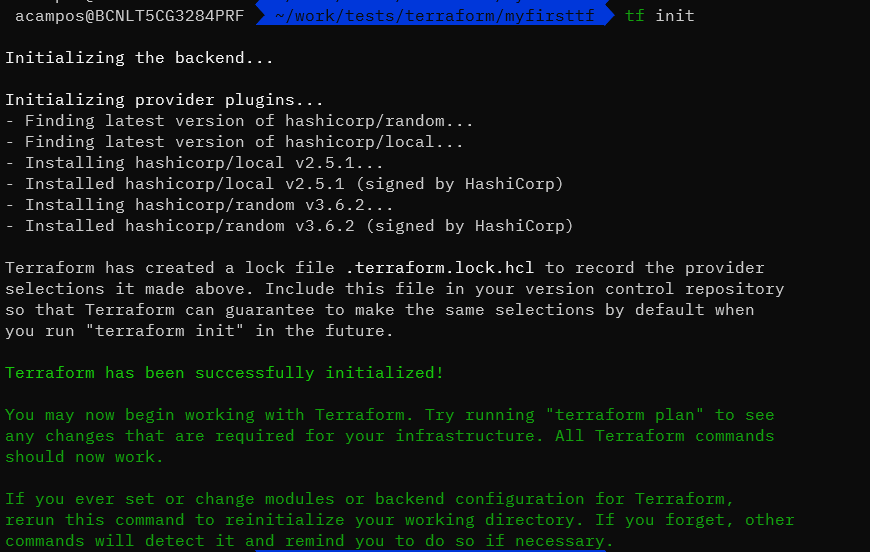
\includegraphics[width=\textwidth]{pictures/pic4.png}
    \centering
\end{figure}
\begin{figure}[H]
    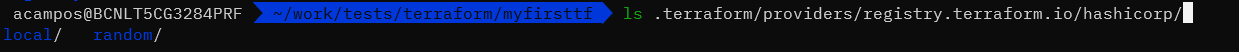
\includegraphics[width=\textwidth]{pictures/pic3.png}
    \centering
\end{figure}
\begin{figure}[H]
    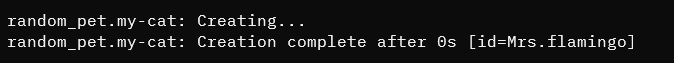
\includegraphics[width=\textwidth]{pictures/pic5.png}
    \centering
\end{figure}

\subsection{Variables in Terraform}

\subsubsection{Basic Variables}

Use variables in code is one of the best practices to can reuse code again and again just configuring a few variables. In case of Terraform, we use variable to configure and deploy resources based on a set of variables that can be provided during the execution. For that purpose, we need to create a new configuration file called \verb+variables.tf+

The \verb+variables.tf+ file, jsut like the \verb+main.tf+ file, consists of blocks and arguments. Let's see an example:

\begin{codetemplate}{variables.tf}
\begin{verbatim}
variable "cats_filename" {
    default = "/tmp/cats.txt"
}

variable "cats_content" {
    default = "I love cats!"
}

variable "my-cat_prefix" {
    default = "Mrs"
}
...
\end{verbatim}
\end{codetemplate}

How to use them? Just replace them by
\begin{codetemplate}{}
\begin{verbatim}
var.cats_filename
\end{verbatim}
\end{codetemplate}

For example:
\begin{codetemplate}{main.tf}
\begin{verbatim}
resource "local_file" "cats" {
    filename = var.cats_filename
    content  = var.cats_content
}

resource "random_pet" "my-cat" {
    prefix = var.my-cat
...  
}
\end{verbatim}
\end{codetemplate}

\begin{blocktemplateIII}{WARNING}
When using variables, you do not have to enclose the values into double quotes ("") as in other IaC programming languages
\end{blocktemplateIII}

Appart from \verb+default+ we can define more arguments for the variables:

\begin{itemize}
    \item \verb+default+: variable value
    \item \verb+description+ (optional): enforces the type of variable
    \item \verb+type+ (optional): what the variable is used for, available types:
    \begin{itemize}
        \item string
        \item number
        \item bool
        \item any
        \item list: \verb+["cat", "dog"]+
        \item map: \verb+{pet1 = cat pet2 = dog}+
        \item object
        \item tuple
    \end{itemize}
\end{itemize}

Simple example:

\begin{codetemplate}{variables.tf}
\begin{verbatim}
variable "length" {
    default     = 2
    type        = number
    description = "length of the pet name"
}

variable "enable_pets" {
    default     = false
    type        = bool
    description = "variable to enable pets"
}
\end{verbatim}
\end{codetemplate}

\begin{blocktemplate}{Note}
As the type is optional, if nothing is specified it is set to type \textbf{any} by default
\end{blocktemplate}

\subsubsection{Lists} 
Numbered collection of values.

\begin{itemize}
    \item Definition
\end{itemize}
\begin{codetemplate}{variables.tf}
\begin{verbatim}
variable "names" {
    default     = ["Mixi", "Nina", "Soda"]
    type        = list
    description = "list of my pet favourite names"
}
\end{verbatim}
\end{codetemplate}
\begin{itemize}
    \item Usage
\end{itemize}
\begin{codetemplate}{main.tf}
\begin{verbatim}
resource "random_pet" "my-cat" {
    prefix = var.names[0]
}
\end{verbatim}
\end{codetemplate}
\begin{itemize}
    \item List of numbers: \verb+type = list(number)+
    \item List of strings: \verb+type = list(string)+
\end{itemize}

\subsubsection{Maps}
Numbered collection of values.

\begin{itemize}
    \item Definition
\end{itemize}
\begin{codetemplate}{variables.tf}
\begin{verbatim}
variable "names" {
    default = {
        "favourite_name": "Nina"
        "other_name": "Mixi"
    }
    type        = map
    description = "my pet favourite names in map"
}
\end{verbatim}
\end{codetemplate}
\begin{itemize}
    \item Usage
\end{itemize}
\begin{codetemplate}{main.tf}
\begin{verbatim}
resource "random_pet" "my-cat" {
    prefix = var.names["favourite_name"]
}
\end{verbatim}
\end{codetemplate}
\begin{itemize}
    \item Map of numbers: \verb+type = map(number)+
    \item Map of strings: \verb+type = map(string)+
\end{itemize}

\subsubsection{Sets} 
Like a list, but without duplicate elements (it is forbiden and \verb+tf apply+ will fail)

\begin{itemize}
    \item Definition
\end{itemize}
\begin{codetemplate}{variables.tf}
\begin{verbatim}
variable "names" {
    default     = ["Mixi", "Nina", "Soda"]
    type        = set(string)
    description = "set of my pet favourite names"
}
\end{verbatim}
\end{codetemplate}
\begin{itemize}
    \item Usage
\end{itemize}
\begin{codetemplate}{main.tf}
\begin{verbatim}
resource "random_pet" "my-cat" {
    prefix = var.names[0]
}
\end{verbatim}
\end{codetemplate}
\begin{itemize}
    \item Set of numbers: \verb+type = set(number)+
    \item Set of strings: \verb+type = set(string)+
\end{itemize}

\subsubsection{Objects} 
Complex data structures by combining all the variable types that we have seen so far

\begin{itemize}
    \item Definition
\end{itemize}
\begin{codetemplate}{variables.tf}
\begin{verbatim}
variable "nina" {
    type = object({
        name          = string
        color         = string
        age           = number
        food          = list(string)
        favourite_pet = bool
    })

    default = {
        name          = "nina"
        color         = "white"
        age           = 3
        food          = ["fish", "meat"]
        favourite_pet = true
    }
    
    description = "nina object definition"
}
\end{verbatim}
\end{codetemplate}

\subsubsection{Tuples} 
Similar to a list; sequence of elements. But the difference is that list uses variables of the same type, such as list of strings, list of numbers, etc. In case of tuple, we can make use of all the elements types.
\begin{itemize}
    \item Definition
\end{itemize}
\begin{codetemplate}{variables.tf}
\begin{verbatim}
variable "kity" {
    type        = tuple([string, number, bool])
    default     = ["Mixi", 7, bool]
    description = "my kity var definition"
}
\end{verbatim}
\end{codetemplate}

\begin{blocktemplateIII}{WARNING}
The order of the elements type should be exactly the same as defined, if not, \verb+tf apply+ will fail
\end{blocktemplateIII}

\begin{itemize}
    \item Usage
\end{itemize}
\begin{codetemplate}{main.tf}
\begin{verbatim}
resource "random_pet" "my-cat" {
    prefix = var.names[0]
}
\end{verbatim}
\end{codetemplate}

\subsubsection{Variables Empty Values Allowed?}
The answer to this question is \textbf{yes}! If you define empty variables when \textbf{tf apply} it will ask you to enter values for each empty variabled defined

\begin{figure}[H]
    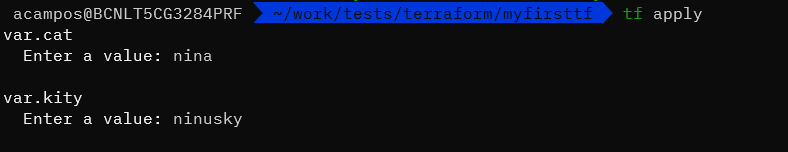
\includegraphics[width=\textwidth]{pictures/pic6.png}
    \centering
\end{figure}

\subsubsection{Variables in Flags}
It is also allowed in Terraform to pass variables as arguments using flags:
\begin{codetemplate}{}
\begin{verbatim}
$ tf apply -var "filename=/tmp/cats.txt" -var "content=I love cats"
\end{verbatim}
\end{codetemplate}

\subsubsection{Terraform Variable Definition Files}
Furthermore, you can define your variables in a file called:
\begin{itemize}
    \item \verb+<file_name>.tfvars+
    \item \verb+<file_name>.tfvars.json+
\end{itemize}

\begin{codetemplate}{terraform.tfvars}
\begin{verbatim}
filename = "/tmp/cats.txt"
content = "I love cats!"
...
\end{verbatim}
\end{codetemplate}

\begin{blocktemplateIII}{WARNING}
The file can be named as you want, but it is mandatory to have one of these both extensions:
\begin{itemize}
    \item \verb+.tfvars+
    \item \verb+.tfvars.json+
\end{itemize}

Then you can pass it as argument to terraform:
\begin{codetemplate}{}
\begin{verbatim}
$ terraform apply -var-file variables.ini
\end{verbatim}
\end{codetemplate}
\end{blocktemplateIII}

\subsubsection{Terraform Variables as Linux env vars}
Terraform is amazing, it is also allowed, you need to define variables as following:
\begin{codetemplate}{}
\begin{verbatim}
$ export TF_VAR_<my_var_name>=<my_var_value>
\end{verbatim}
\end{codetemplate}

\subsubsection{Terraform Variables Definition Precedence}
\begin{enumerate}
    \item Variables in flags.
    \item Terraform Variable Definition File (specified in \verb+-var-file+).
    \item Terraform Variable Definition File (default ones).
    \item Linux Enviroment Variables.
\end{enumerate}


\subsection{Reference Attributes}
There are a lot of resources that are dependent on each other, for example imaginte that we want to make use of the output of one resource and use it as an input for another one?

If we go to the documentation of the providers, we will see a section called \textbf{Schema}, where we will see a list of attributes returned back from the resource after you run \verb+tf apply+.

If we look at the example before, \verb+random_pet+ resource returns just one attribute called \textbf{id (string)}

\begin{figure}[H]
    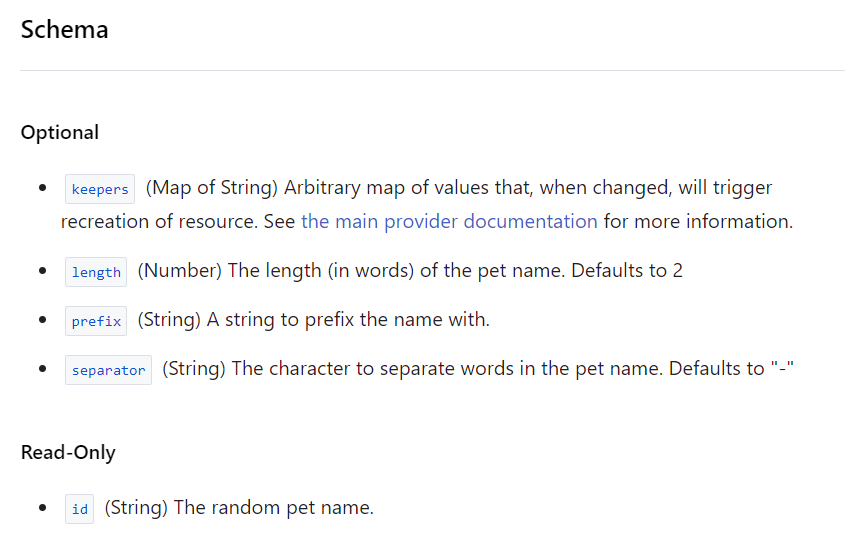
\includegraphics[width=\textwidth]{pictures/pic7.png}
    \centering
\end{figure}

So, we can link one resource to another using reference attributes:

\begin{codetemplate}{main.tf}
\begin{verbatim}
resource "local_file" "cats" {
    filename = var.cats_filename
    content  = random_pet.my-cat.id
}
    
resource "random_pet" "my-cat" {
    prefix    = var.names[0]
    separator = var.separator
    length    = var.length
}
\end{verbatim}
\end{codetemplate}

If we want to include it into an string:
\begin{codetemplate}{main.tf}
\begin{verbatim}
resource "local_file" "cats" {
    filename = var.cats_filename
    content  = "My pet is called ${random_pet.my-cat.id}"
}
    
resource "random_pet" "my-cat" {
    prefix    = var.names[0]
    separator = var.separator
    length    = var.length
}
\end{verbatim}
\end{codetemplate}

If you run \verb+tf apply+ you will see the variable replaced!

\subsubsection{Resource Dependency}
When Terraform creates these resoruces, it knows about the dependencies of the resources. So if we follow the example before, Terraform knows that \verb+local_file+ depends on \verb+random_pet+, so as a result, it uses the appropiate order to provision resources. Besides, when resources are deleted, Terraform does it in the inverse order.

As well, if we don't have any dependency relation but we want to stablish it, in order to force the order Terraform creates the resources, we can do it using \textbf{explicit dependencies}:

\begin{codetemplate}{main.tf}
\begin{verbatim}
resource "local_file" "cats" {
    filename   = var.cats_filename
    content    = "My pet is called Nina"
    depends_on = [
        random_pet.my-cat
    ]
}
    
resource "random_pet" "my-cat" {
    prefix    = var.names[0]
    separator = var.separator
    length    = var.length
}
\end{verbatim}
\end{codetemplate}

Resource dependency is a very important feature in Terraform, so it is common to need some order in the configuration / deployment of your infrastructure, so you need one resource to not be created until another one is. If dependencies are not explicit or implicit defined, Terraform will do it randomly parallelizing as much as he can with the resource creation / update.

\subsubsection{Output Variables}
Along with input variables, Terraform also supports output variables, this variables can be used to store the value of an expression in Terraform. So we can assign the value of the output of a function to a variable:

\begin{codetemplate}{main.tf}
\begin{verbatim}
resource "random_pet" "my-cat" {
    prefix    = var.names[0]
    separator = var.separator
    length    = var.length
}

output "pet_name" {
    value = random_pet.my-cat.id
    description = "Record the value of pet ID generated 
                    by the random_pet resource"
}
\end{verbatim}
\end{codetemplate}

To se the values of the output variables we can run:
\begin{itemize}
    \item To see al the output variables
\end{itemize}
\begin{codetemplate}{}
\begin{verbatim}
$ terraform output
\end{verbatim}
\end{codetemplate}
\begin{itemize}
    \item To see an specific variable
\end{itemize}
\begin{codetemplate}{}
\begin{verbatim}
$ terraform output <output_variable_name>
\end{verbatim}
\end{codetemplate}
\begin{itemize}
    \item When you run \verb+tf apply+ it also display the output variable values
\end{itemize}

We already saw that dependent resources can make use of reference expressions to get the output from one resource block as an input to another block. As such, output variables are not really required here. The mainly usage of output variables is when you want to quickly display details about a provision resource on the screen, or to feed the output variables to other IaC tools.

\begin{blocktemplateIII}{WARNING}
We need to first \verb+tf apply+, if not, any variable will be printed on the \verb+tf output+
\end{blocktemplateIII}

%====================================================================================================
\newpage
\section{Terraform State}

\subsection{Introduction}
In this section we are going to discover what Terraform State is and see what really happens under the hoods when we run terraform commands. When we run \verb+terraform apply+ the first action Terraform does is to check if there are some past states of this resource stored in-memory. If it does not find any on the memory it will implement the creation of the resource.

As well, \verb+terraform apply+ tries to refresh the in-memory state, and when applied, it assigns to the resources unique \textbf{id's}, so next time we try to apply changes using terraform, it will know the configuration on the resource. It is done creating a file inside the directory called: \verb+terraform.tfstate+, this file is a JSON data structure that maps the real-world infrastructure resources to resource definition in the configuration files, it has all the record of the infrastructure created by this Terraform directory:

\begin{figure}[H]
    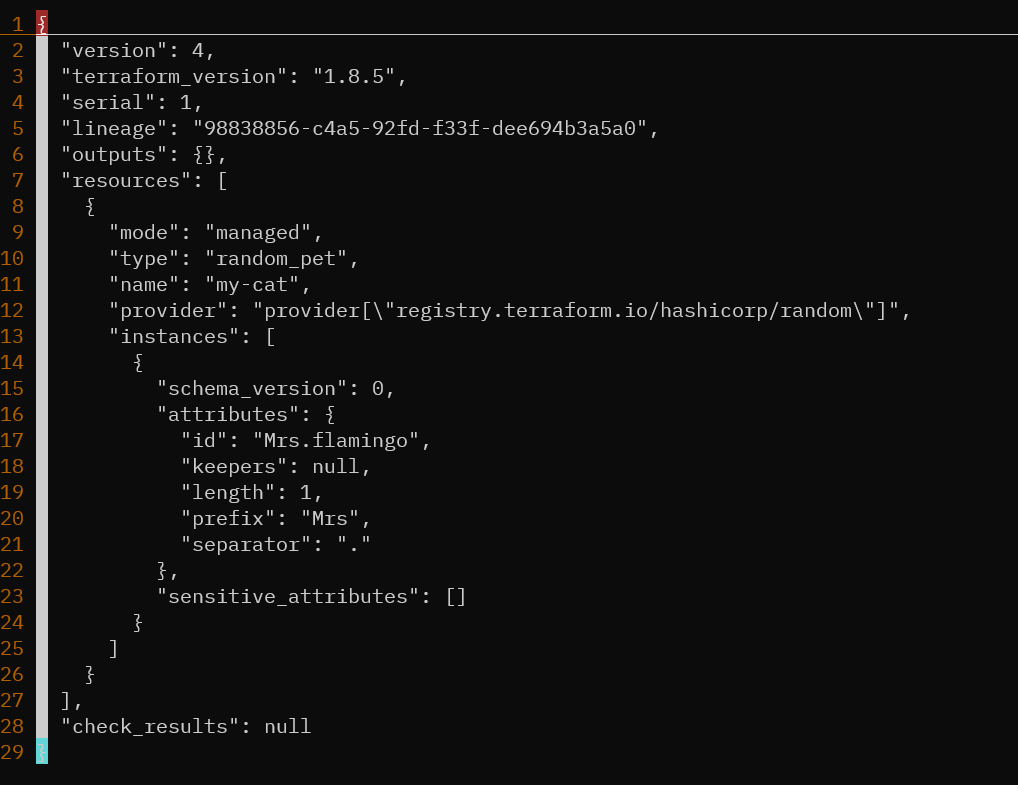
\includegraphics[width=\textwidth]{pictures/pic8.png}
    \centering
\end{figure}

\verb+terraform.tfstate+ file contains every little detail belonging to the infrastructure that was created by Terraform on this directory. It uses it as a single source of truth when using commands such as \verb+terraform plan+ and \verb+terraform apply+. So each time we apply new changes using Terraform:
\begin{enumerate}
    \item Terraform check the state of the resources checking this file
    \item Terraform change this file to record new state of the resources, if the resource is unmutable, it will generate a new \textbf{id} for the resource, if not, it will keep the old one.
\end{enumerate}

So Terraform uses \verb+.tfstate+ file to map the resources configuration with the real world infrastructure, and this mapping allows Terraform to create execution plans when a drift is identify between the resources configuration file and the statefile. It also tracks resource metadata such as resource dependencies.

\subsection{Forcing Terraform to believe in .tfstate file}
When dealing with a handful number of resources, it may be feasible for Terraform to reconcile state with the realworld infrastructure after every single terraform command (pla/apply). But Terraform use to manage a lot of resources, and resources distributed for different providers. So it is not feasible for Terrafomr to reconcile state for every terraform resource, that's why it can take long times to perform the actions.

So in the cases that Terraform takes a lot to perform \verb+tf plan+ or \verb+tf apply+ you can make the \verb+.tfstate+ file as the only record of truth, \textbf{without having to reconcile}, improving the performance significantly. 

To do this:
\begin{codetemplate}{}
\begin{verbatim}
$ terraform plan -refresh=false
\end{verbatim}
\end{codetemplate}

\subsection{How to share State File between team members?}
As you already know, Terraform stores the changes applied to the \verb+terraform.tfstate+ file, which is stored locally in the same directory you run Terraform. That's good for starting projects, but what about shared projects working with more than one person? Every user in the team should always have the latest state data before running Terraform, and make sure that nobody else runs Terraform at the same time.

So it is highly recommended to save the \verb+terraform.tfstate+ file in a remote data store rather than to rely on a local copy. This allows the state to be shared between all members of the team.

But we must consider that \verb+terraform.tfstate+ contains sensitive information, within it contains every little detail about our infrastructure: as private and public IP's, cpu's, size and type of disks, ssh keypad, initial database passwords, etc. And as you can see, it is stored as a basic JSON format file, so it should be encrypted and stored in a secure storage, \textbf{so it is NOT recommended to store it on git public repositories}. Instead, you should store the state in remote backend systems like:
\begin{itemize}
    \item AWS S3
    \item Google Cloud Storage
    \item HasiCorp Consul
    \item Terraform Cloud
\end{itemize}

%====================================================================================================
\newpage
\section{Deeping on Terraform}

\subsection{Terraform Commands}
To check syntax: 
\begin{codetemplate}{}
\begin{verbatim}
$ terraform validate
\end{verbatim}
\end{codetemplate}

To scan the configuration files and formats the code into a canonical format:
\begin{codetemplate}{}
\begin{verbatim}
$ terraform fmt
\end{verbatim}
\end{codetemplate}

To take a look on the current state of the infrastructure as seen by Terraform:
\begin{codetemplate}{}
\begin{verbatim}
$ terraform show [-json]
\end{verbatim}
\end{codetemplate}

To list all providers used in the configuration files:
To check syntax: 
\begin{codetemplate}{}
\begin{verbatim}
$ terraform providers
\end{verbatim}
\end{codetemplate}

To print all the output variables:
\begin{codetemplate}{}
\begin{verbatim}
$ terraform output [var_name]
\end{verbatim}
\end{codetemplate}

To sync Terraform with the real world infrastructure, to take into account changes made to a resource created by Terraform outside its control (as manual changes). This reconciliation is useful to determine what action to take during the next apply. It doesn't modify any resource but it modifies the state file:
\begin{codetemplate}{}
\begin{verbatim}
$ terraform refresh
\end{verbatim}
\end{codetemplate}

\begin{blocktemplateII}{Note}
The \verb+tf refresh+ command is run automatically when running other Terraform commands such as \verb+tf plan+ and \verb+tf apply+. But it can be bypassed as we have seen before using the \verb+-refresh=false+ flag.
\end{blocktemplateII}

To create a visual representation of the dependencies and a Terraform configuration or an execution plan:
\begin{codetemplate}{}
\begin{verbatim}
$ terraform graph
\end{verbatim}
\end{codetemplate}

\begin{blocktemplateI}{Note}
The output make no much sense, but we can visualize it doing:
\begin{enumerate}
    \item Install visualized in Linux like graphviz
\begin{codetemplate}{}
\begin{verbatim}
$ apt install graphviz -y
\end{verbatim}
\end{codetemplate}
    \item The execute the terraform
\begin{codetemplate}{}
\begin{verbatim}
$ tf graph | dot -Tsvg > graph.svg
\end{verbatim}
\end{codetemplate}
    \item Download the file and open it in a browser
\end{enumerate}
\end{blocktemplateI}

\subsection{Mutable vs Immutable Infrastructure}
mutable infrastructure refers to a system where components can be updated or modified after their initial creation. This traditional approach involves making changes directly to the existing infrastructure. For instance, if a server needs a software update or configuration change, these modifications are applied directly to the live server. 

However, this approach can lead to configuration drift, where the actual state of the infrastructure diverges from the defined configuration over time, potentially leading to inconsistencies and hard-to-debug issues.

mmutable infrastructure, on the other hand, promotes a paradigm where components are never modified after their creation. Instead of updating an existing resource, a new instance is created with the desired changes, and the old one is replaced. This ensures that the infrastructure's state remains consistent and predictable, aligning closely with the declarative nature of Terraform. With immutable infrastructure, if an application or server needs an update, a new version of the server is created with the updates, and the old version is decommissioned. This approach significantly reduces the risk of configuration drift and makes rollbacks straightforward, as reverting to a previous state is simply a matter of redeploying the previous version of the infrastructure.

\begin{blocktemplateIII}{WARNING}
Furthermore, by default Terraform destroys the resource first before creating a new one in its place!! So if the creation failed, the previous resource would be removed and not replaced XD
\\\\
But, we can change this behaviour with \textbf{LifeCycle Rules}
\end{blocktemplateIII}

\subsection{LefeCycle Rules}
Previously we have seen that when Terraform updates an immutable resource first deletes the resource before creating a new one with the updated configuration. But this may not be a desirable approach in all cases, and omsetimes you may want the updated version of the resource to be created first before the older one is deleted, or you may not want the resource to be deleted at all, even if there was a change made in its local configuration. This can be achieved in Terraform by using Lifecycle Rules.

Lifecycle Rules make use of the same block syntax that we have seen many times so far, and they go directly inside the resource block whose behavior we want to change. For example:

\begin{codetemplate}{main.tf}
\begin{verbatim}
resource "local_file" "cats" {
    filename = var.cats_filename
    content  = "My pet is called Nina"
    
    lifecycle {
        create_before_destroy = true
    }
}
\end{verbatim}
\end{codetemplate}

To create the resource replacement before removing:
\begin{codetemplate}{main.tf}
\begin{verbatim}
lifecycle {
    create_before_destroy = true
}
\end{verbatim}
\end{codetemplate}

\begin{blocktemplateIII}{WARNING}
Be carefull applying this lifecycle rule, because if we apply it for example to a \verb+local_file+, the local file, we are saying to Terraform to create first a file in a location, and then the same file to be destroyed in the same location during the recreate operation. This goes to show that it is not always advisable to use this rule!
\end{blocktemplateIII}

To avoid the destruction of a resource:
\begin{codetemplate}{main.tf}
\begin{verbatim}
lifecycle {
    prevent_destroy = true
}
\end{verbatim}
\end{codetemplate}

\begin{figure}[H]
    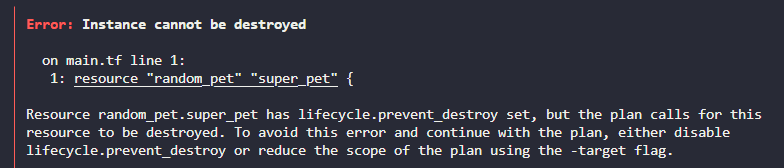
\includegraphics[width=\textwidth]{pictures/pic11.png}
    \centering
\end{figure}

\begin{blocktemplateIII}{WARNING}
This resources are not destroyed if we use \verb+tf apply+ command, but they can be destroyed running the \verb+tf destroy+ command
\end{blocktemplateIII}

To prevent a resource from being updated:
\begin{codetemplate}{main.tf}
\begin{verbatim}
lifecycle {
    ignore_changes = all
}
\end{verbatim}
\end{codetemplate}

To prevent a resource from being updated if one or more atributes are modified (but not all):
\begin{codetemplate}{main.tf}
\begin{verbatim}
lifecycle {
    ignore_changes = [
        <atribute1>,
        <atribute2>,
    ]
}
\end{verbatim}
\end{codetemplate}

\subsection{Datasources}
Imagine that a databse instance was provisioned manually in the AWS Cloud, although Terraform does not manage this resource, it can read atributes  such as the database name, host address, or the DB user. And can use this data to privison an application resource that is managed by Terraform using \textbf{datasources}

Let's see an example of how the content of the resource in \verb+/tmp/dog.txt+ not managed by Terraform can be used to fulfill the \verb+/tmp/cat.txt+

\begin{codetemplate}{main.tf}
\begin{verbatim}
resource "local_file" "cats" {
    filename = var.cats_filename
    content  = data.local_file.dog.content
}

data "local_file" dog" {
    filename = "/tmp/dog.txt"
} 
\end{verbatim}
\end{codetemplate}

The datasources you can extract of each resource can be found on the documentation of each provider and resource type:

\begin{figure}[H]
    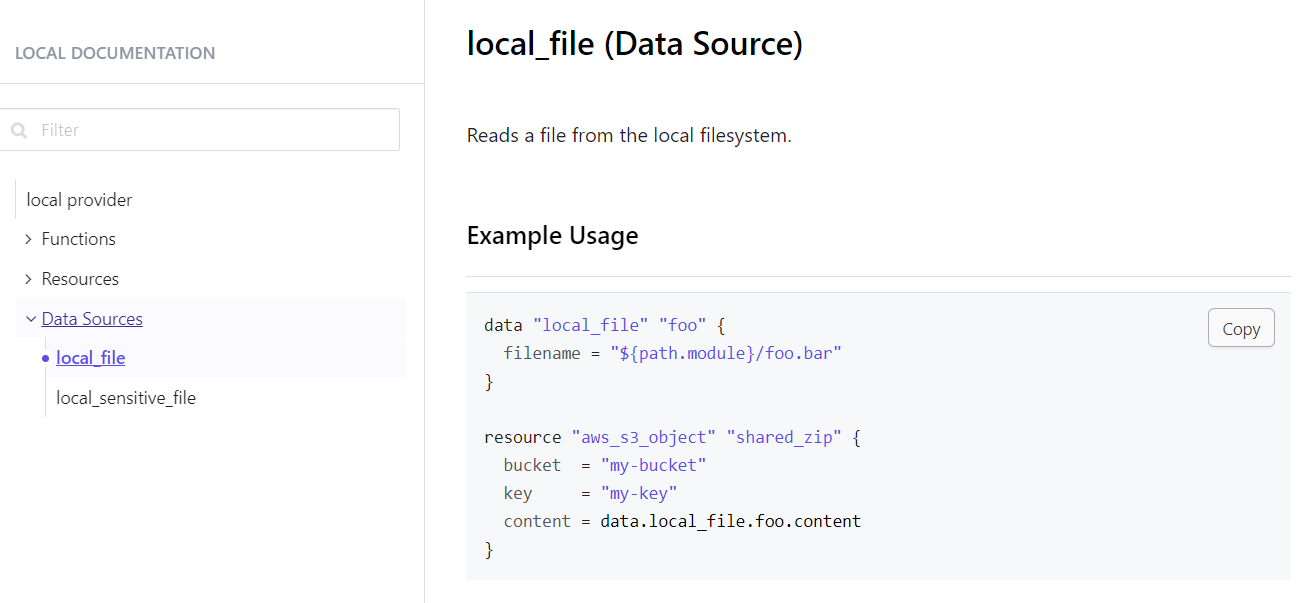
\includegraphics[width=\textwidth]{pictures/pic9.png}
    \centering
\end{figure}

\begin{blocktemplateI}{Note}
Do not confuse resources with datasources! 
\begin{itemize}
    \item Resources are created with the \verb+resource+ block, they are use to create, update and destroy infrastructure.
    \item Datasources are crerated with the \verb+data+ block, they are used to read information from a specific resource.
\end{itemize}
\end{blocktemplateI}


\subsection{Meta Arguments}
So far, we have seen how to create individual resources, but what if we want to create multiple instance of the same resource? So using \textbf{Meta Arguments}. We have defined two Meta Arguments during this course:

\subsubsection{Depends On}
\begin{codetemplate}{main.tf}
\begin{verbatim}
depends_on = [
    random_pet.my-pet
]
\end{verbatim}
\end{codetemplate}

\subsubsection{Lifecycle}
\begin{codetemplate}{main.tf}
\begin{verbatim}
lifecycle {
    prevent_destroy = true
}
\end{verbatim}
\end{codetemplate}

\subsubsection{Count}

\begin{codetemplate}{main.tf}
\begin{verbatim}
count = #Number_of_instances
\end{verbatim}
\end{codetemplate}

In the following example terraform will try to create the same file 3 times:
\begin{codetemplate}{main.tf}
\begin{verbatim}
resource "local_file" "cats" {
    filename = "/tmp/cats.txt"
    content  = "My pet is called Nina"
    count    = 3
}
\end{verbatim}
\end{codetemplate}

To create 3 different resources:
\begin{codetemplate}{main.tf}
\begin{verbatim}
resource "local_file" "cats" {
    filename = var.filename[count.index]
    content  = "My pet is called Nina"
    count    = length(var.filename)
}

variable "filename" {
    type    = list(string)
    default = [
        "/tmp/cats.txt",
        "/tmp/dogs.txt",
        "/tmp/pets.txt
    ]
}
\end{verbatim}
\end{codetemplate}

\begin{blocktemplateII}{Note}
Also we have used a built in Terraform function: \verb+length()+ which will return the length of a list, set or map.
\end{blocktemplateII}

\begin{blocktemplateIII}{WARNING}
Use \verb+count+ is not a good practice in Terraform, because if we want to remove one of the elements on the list it will probably destroy and recreate all the following elements. Because it detects that are not on the same possition on the list. So avoid as much as you can use this and use \verb+for_each+ instead.
\end{blocktemplateIII}

\subsection{For Each}
This is the best way to create multiple instance of the same resource in Terraform. Because it will not remove any resource extra if we just want to remove one of the resources and you can add as many resources as you want.

\begin{codetemplate}{main.tf}
\begin{verbatim}
resource "local_file" "cats" {
    for_each = var.filename    

    filename = each.value
}

variable "filename" {
    type    = set(string)
    default = [
        "/tmp/cats.txt",
        "/tmp/dogs.txt",
        "/tmp/pets.txt
    ]
}
\end{verbatim}
\end{codetemplate}

\newpage
\begin{blocktemplateIII}{WARNING}
The \verb+for_each+ Meta Argument only works with \textbf{maps} or \textbf{sets}. Because using \verb+for_each+ Terraform is converting the variable into a \verb+map+ so the resources are no longer identified by the index, they are identified by its value, to avoid the same missbehaviout as \verb+count+. That's why we changed the \verb+filename+ variable to a type set.
\\\\
Also we could do the following using the built in Terraform function: \verb+toset()+ which will convert a list to a set.

If we look now to the variable, it is converted to a map:

\begin{codetemplate}{main.tf}
\begin{verbatim}
resource "local_file" "cats" {
    for_each = toset(var.filename)

    filename = each.value
}

variable "filename" {
    type    = list(string)
    default = [
        "/tmp/cats.txt",
        "/tmp/dogs.txt",
        "/tmp/pets.txt"
    ]
}
\end{verbatim}
\end{codetemplate}

\begin{figure}[H]
    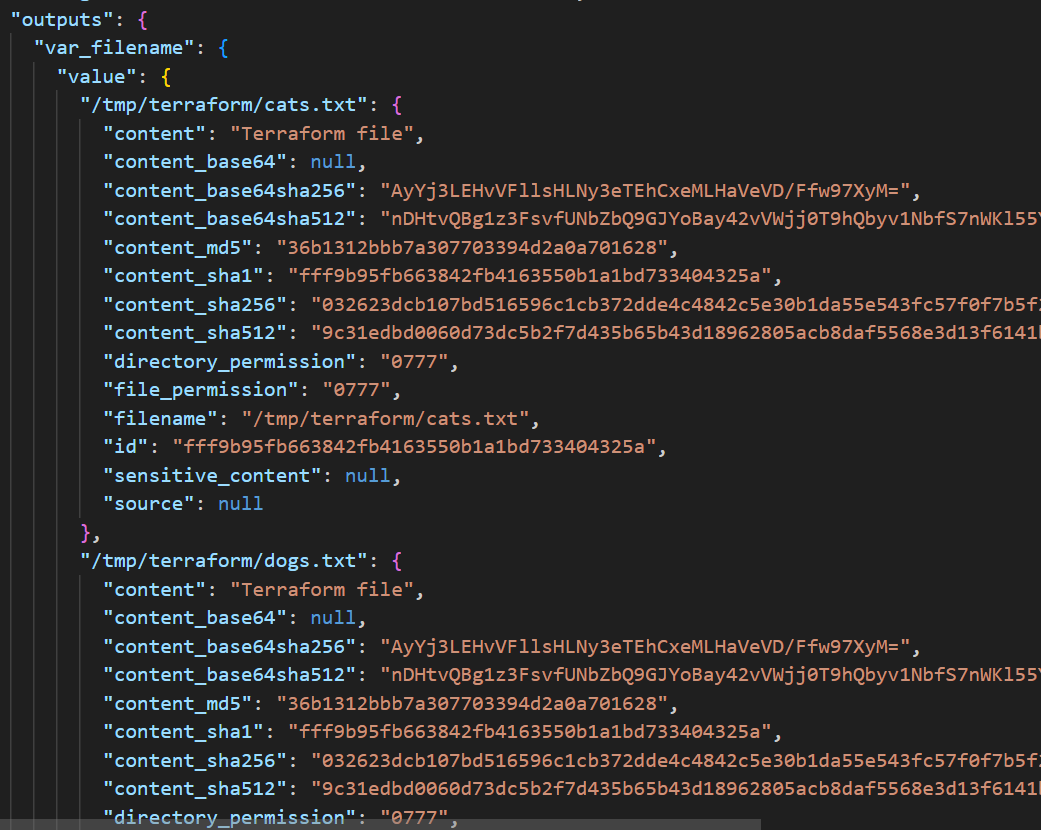
\includegraphics[width=\textwidth]{pictures/pic10.png}
    \centering
\end{figure}
\end{blocktemplateIII}

\subsection{Version Constraints}
In this section we will see how to make use of specific provider versions in Terraform. Without specific configuration, \verb+tf init+ command downloads the latest version of the provider plugins that are needed by the configuration files. The instructions to use a specific version of a provider is available in the provider documentation in the registry.

\begin{figure}[H]
    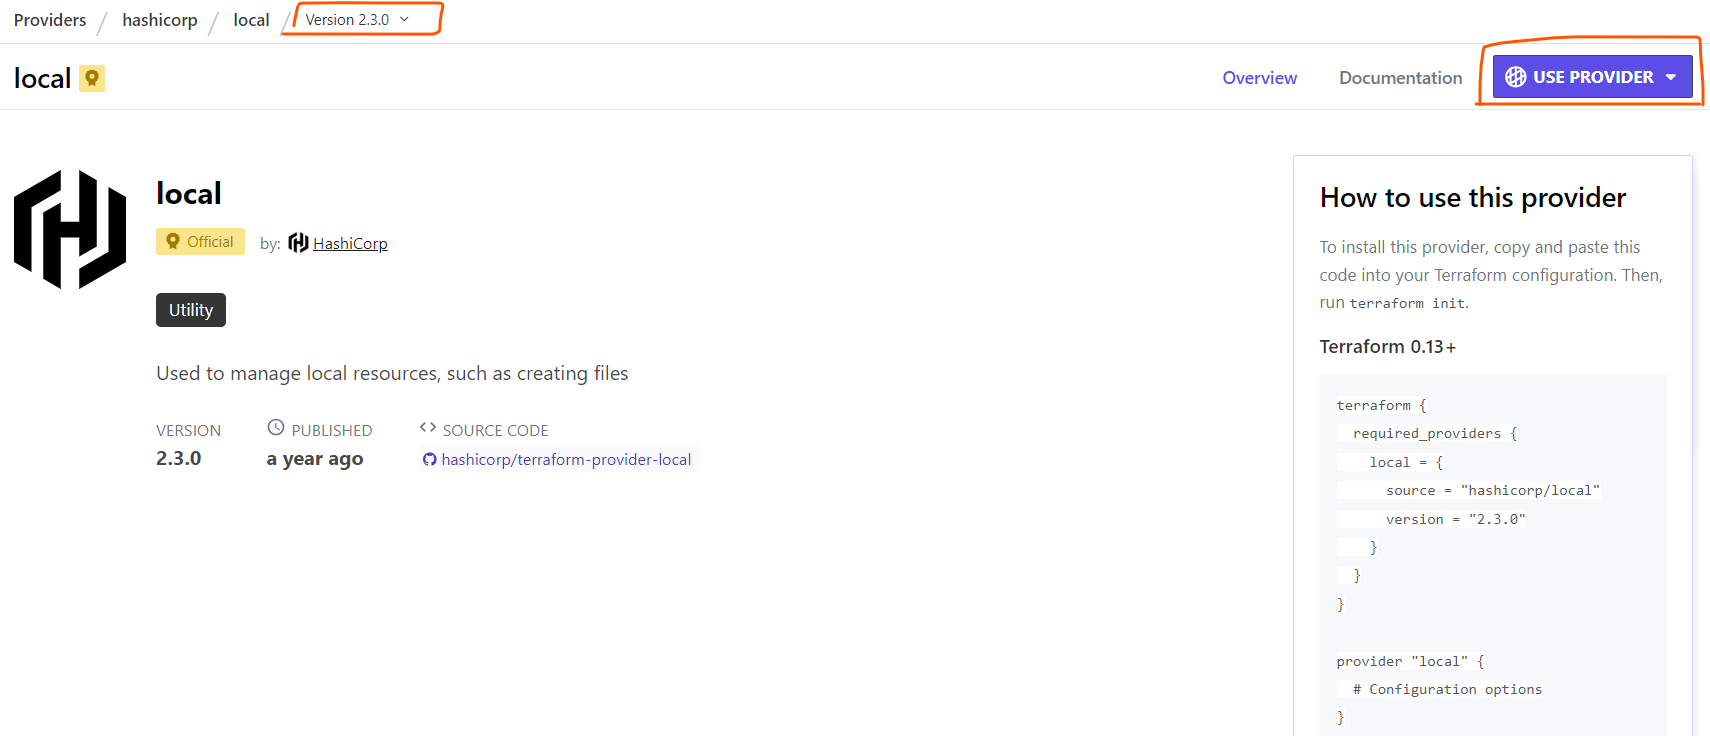
\includegraphics[width=\textwidth]{pictures/pic12.png}
    \centering
\end{figure}

So of you have seen, to define the version of a specific provider we will need to use a new block: \verb+required_providers+ under \verb+terraform+ block:

\begin{codetemplate}{providers.tf}
\begin{verbatim}
terraform {
    required_providers {
        local = {
           source = "hashicorp/local"
           version = "2.3.0"
        }
    }
}
\end{verbatim}
\end{codetemplate}

We can use more version constrains:
\begin{codetemplate}{providers.tf}
\begin{verbatim}
terraform {
    required_providers {
        local = {
           source = "hashicorp/local"
           version = "!= 2.3.0"
        }
    }
}
\end{verbatim}
\end{codetemplate}

\begin{blocktemplate}{Note}
To configure providers, it is common to create a new file to write this configuration:
\begin{codetemplate}{}
\begin{verbatim}
providers.tf
\end{verbatim}
\end{codetemplate}
\end{blocktemplate}

\begin{codetemplate}{providers.tf}
\begin{verbatim}
terraform {
    required_providers {
        local = {
            source = "hashicorp/local"
            version = "< 2.3.0"
        }
    }
}
\end{verbatim}
\end{codetemplate}

\begin{codetemplate}{providers.tf}
\begin{verbatim}
terraform {
    required_providers {
        local = {
            source = "hashicorp/local"
            version = "> 2.3.0"
        }
    }
}
\end{verbatim}
\end{codetemplate}

\begin{codetemplate}{providers.tf}
\begin{verbatim}
terraform {
    required_providers {
        local = {
            source = "hashicorp/local"
            version = "~> 2.3.0"
        }
    }
}
\end{verbatim}
\end{codetemplate}

\begin{codetemplate}{providers.tf}
\begin{verbatim}
terraform {
    required_providers {
        local = {
            source = "hashicorp/local"
            version = "> 2.3.0, < 3.0.0, != 2.5.0"
        }
    }
}
\end{verbatim}
\end{codetemplate}

%====================================================================================================
\newpage
\section{Terraform with AWS}
AWS is one of the most popular cloud computing platforms in the world offering hundreds of services, such as:
\begin{itemize}
    \item Compute
    \item DB's
    \item Storage
    \item Machine Learning
    \item Analytics
    \item Iot
\end{itemize}

Having all this infrastructure options it make the companies easier to build their applications on AWS or migrate its on-premiss infrastructure to AWS. Also, it has the most extensive global cloud infrastructure, this allows us to deploy services in a number of different globally distribution regions, and within multiple datacenters known as availability zones.

\subsection{Introduction to IAM (Identity and Access Management)}
The account you created at frist time using AWS is an administrator account, you can manage any service within AWS using this account, but this is not the recommended approach. This user account can be compared with \verb+root+ account in Linux. So the best practice is to create new users with different permissions using this root account, and do not use the root account for any other purpose.

When we create users in AWS there are 2 types of access that we can configure:

\begin{itemize}
    \item Access to the management console (user and password) to access the GUI
    \item Programmatic access (key value ID-secret) to use terminal
\end{itemize}

With IAM, you can set permissions for other users to access, view, edit, the resources. And as well roles can be managed to enable the access between different services on AWS:

\subsection{Accessing AWS Programmaticaly}
\begin{enumerate}
    \item Create a programatic access through the GUI
    \item Install aws binary
\begin{codetemplate}{}
\begin{verbatim}
$ curl "https://awscli.amazonaws.com/awscli-exe-linux-x86_64.zip" -o "awscliv2.zip"
  unzip awscliv2.zip
  sudo ./aws/install
\end{verbatim}
\end{codetemplate}

    \item Configure aws binary, it will ask for the key-secret generated on the GUI
\begin{codetemplate}{}
\begin{verbatim}
$ aws configure
\end{verbatim}
\end{codetemplate}
\end{enumerate}
\begin{blocktemplateI}{Note}
As output format you can choose JSON, YAML, TXT or Table, but it is recommended to choose JSON.
\\\\
The configuration is stored under \verb+~/.aws/config+
\end{blocktemplateI}

Basic Usage of aws cli:
\begin{codetemplate}{}
\begin{verbatim}
$ aws <command> <subcommand> [parameters]
\end{verbatim}
\end{codetemplate}

\begin{codetemplate}{}
\begin{verbatim}
$ aws help
\end{verbatim}
\end{codetemplate}

\begin{codetemplate}{}
\begin{verbatim}
$ aws <command> help
\end{verbatim}
\end{codetemplate}

\begin{codetemplate}{}
\begin{verbatim}
$ aws <command> <subcommand> help
\end{verbatim}
\end{codetemplate}

Some examples:
\begin{itemize}
    \item Create a user
\end{itemize}
\begin{codetemplate}{}
\begin{verbatim}
$ aws iam create-user --user-name lucy
\end{verbatim}
\end{codetemplate}
\begin{itemize}
    \item Create a group
\end{itemize}
\begin{codetemplate}{}
\begin{verbatim}
$ aws iam create-group --group-name lucy
\end{verbatim}
\end{codetemplate}
\begin{itemize}
    \item Create a group
\end{itemize}
\begin{codetemplate}{}
\begin{verbatim}
$ aws iam create-group --group-name lucy
\end{verbatim}
\end{codetemplate}

\begin{blocktemplate}{Note}
When you create a resource on AWS, an \verb+ARN+ will be assigned to it, and it is the unique id assigned to each resource on AWS.
\end{blocktemplate}

\subsection{IAM resources with Terraform}

\href{https://registry.terraform.io/providers/hashicorp/aws/latest}{Official AWS Provider Documentation}

The first thing we need to do is configure the provider:

\begin{codetemplate}{}
\begin{verbatim}
provider "aws" {
    region = "us-west-2"
    access_key = "fdjhsakfhas"
    secret_key = "fhhashfakshl"
}
\end{verbatim}
\end{codetemplate}

\begin{blocktemplateIII}{WARNING}
This is not a good practice, it is better to store this data in your machine using \verb+aws configure:+
\begin{itemize}
    \item \verb+~/.aws/config+
    \item \verb+~/.aws/credentials+
\end{itemize}
\begin{codetemplate}{}
\begin{verbatim}
[default]
aws_access_key_id =
aws_secret_access_key =
\end{verbatim}
\end{codetemplate}

Another option is to define the following variables:
\begin{codetemplate}{}
\begin{verbatim}
$ export AMS_ACCESS_KEY_ID=
  export AMS_SECRET_ACCESS_KEY_ID=
  export AMS_REGION=
\end{verbatim}
\end{codetemplate}

\end{blocktemplateIII}

The we should define the iam resource we want to add:
\begin{codetemplate}{}
\begin{verbatim}
resource "aws_iam_user" "lucy_user" {
    name = "lucyr"
    path = "/system/"
    
    tags = {
        description = "Technical Team Lead"
    }
}
\end{verbatim}
\end{codetemplate}

\subsection{IAM Policies with Terraform}
In this section we will se how to create IAM policies with Terraform and attach them to users and groups.

\begin{blocktemplateII}{Note}
All users in AWS start with the least privileges. To add permissions we need to add policies to groups and users.
\end{blocktemplateII}

For example:

\begin{codetemplate}{}
\begin{verbatim}
resource "aws_iam_policy" "admin_policy" {
    name   = "AdminUsers"
    policy = <<EOF
    {
        Version   = "2012-10-17"
        Statement = [
          {
            Action = [
              "ec2:Describe*",
            ]
            Effect   = "Allow"
            Resource = "*"
          },
        ]
    }
    EOF
}

resource "aws_iam_user_policy_attachment" "lucy_admin_access" {
    user       = aws_iam_user.lucy_user.name
    policy_arn = aws_iam_policy.admin_policy.arn
}
\end{verbatim}
\end{codetemplate}

Another way to specify the policy is:

\begin{codetemplate}{admin-policy.json}
\begin{verbatim}
{
    Version = "2012-10-17"
    Statement = [
        {
        Action = [
            "ec2:Describe*",
        ]
        Effect   = "Allow"
        Resource = "*"
        },
    ]
}
\end{verbatim}
\end{codetemplate}
\begin{codetemplate}{}
\begin{verbatim}
resource "aws_iam_policy" "admin_policy" {
    name   = "AdminUsers"
    policy = file("admin-policy.json")
}

resource "aws_iam_user_policy_attachment" "lucy_admin_access" {
    user       = aws_iam_user.lucy_user.name
    policy_arn = aws_iam_policy.admin_policy.arn
}
\end{verbatim}
\end{codetemplate}

\subsection{Introduction to S3 in AWS}
S3 stands for a Simple Storage Service in AWS, insted it is simple, it provides infinitely scalable storage solution from AWS. Also offering high availablility of data storing it in across multiple devices and availability zones in a region. S3 is an object base storage, it allows us to store objects or flat files, such as documents, images and videos in the AWS cloud. It is equivalent to a file share storage, such as NFS, which are suitable to install flat files but not to install OS or DB's. 

Data in S3 is stored in the form of an S3 bucket, a bucket can be considered to be a container of a directory which stores all your files, and you can create as many as this buckets as you wish in your AWS account. Everything within a bucket is an object, so imagine that we have an S3 bucket called "pets".

\begin{codetemplate}{pets}
\begin{verbatim}
lolo.txt
pictures/
    |-- nina.mp4
    |-- set.mp4
videos/
    |-- nina.mp4
    |-- set.mp4
\end{verbatim}
\end{codetemplate}

Every item (files and folders) is an object, so the files are objects, and the files inside folders are objects wiht the fullpath, and also the folders are objects.

When you create a bucket on AWS, the \textbf{bucket name} must be unique, because once it is created, AWS creates also a DNS name for it, accessible from anywhere in the world. So, the name should be as well dns compliant: no uppercases, no underscores and between 3 and 63 characters long. When the bucket is created it will be accessible through the DNS name which looks like this:
\begin{codetemplate}{}
\begin{verbatim}
https://<bucket_name>.<region>.amazonaws.com
\end{verbatim}
\end{codetemplate}  

Also any object inside the bucket is accessible through:
\begin{codetemplate}{}
\begin{verbatim}
<bucket_dns>/path
\end{verbatim}
\end{codetemplate} 

Any object in an S3 bucket consists of an object data and metadata: 
\begin{itemize}
    \item \textbf{Data}
    \begin{itemize}
        \item \textbf{key:} actual name of the object
        \item \textbf{value:} actual data referenced by that object
    \end{itemize}

    \item \textbf{Metadata:} details about the object stored in the bucket
    \begin{itemize}
        \item The time when the object was created
        \item The owner of the object
        \item The size of the object
        \item ...
    \end{itemize}
\end{itemize}

When an object is uploaded to an AWS bucket, it provides it the least permissions. So by default, no one can access the objects in the bucket with the exception of the bucket owner. Access to the bucket permissions are managed through \textbf{bucket policies}, and the bucket objects specific permissions are manage through \textbf{access control lists}

\subsection{S3 with Terraform}
Let's create 2 resources in AWS: a bucket and a bucket object:
\begin{codetemplate}{main.tf}
\begin{verbatim}
resource "aws_s3_bucket" "terraform_learning" {
    bucket = "terraform-learning-242384230"
    tags   = {
        description = "Files regarding terraform learning"
    }
}

resource "aws_s3_bucket_object" "terraform_basis" {
    content = "/path/to/your/local/file"
    key     = "terraform_basis.txt"
    bucket  = aws_s3_bucket.terraform.id
}
\end{verbatim}
\end{codetemplate}

Now define the policies and set them:
\begin{codetemplate}{main.tf}
\begin{verbatim}
data "aws_iam_group" "terraform_students" {
    group_name = "terraform_students"
}

resource "aws_s3_bucket_policy" "terraform_students_policy" {
    bucket  = aws_s3_bucket.terraform.id
    policy = <<EOF
    {
        Version   = "2012-10-17"
        Statement = [
          {
            "Action" = "*",
            "Effect"   = "Allow",
            "Resource" = "arn:aws:s3:::${aws_s3_bucket.terraform.id}/*"
            "Principal": {
                "AWS": [
                    "${data.aws_iam_group.terraform_students.arn}"
                ]
            }
          }
        ]
    }
    EOF
}
\end{verbatim}
\end{codetemplate}

\subsection{Introduction to DynamoDB in AWS}
DynamoDB is a no SQL database solution provided by AWS, it is a highly scalable database that can cope with millions of requests from applications such as mobile, web, gaming, iot, etc. It is a fully managed service from AWS. It provides high availability (because the data is replicated across different AWS regions), easy scalability and low latency data access. 

A no SQL database are those which store the data in key-value pairs and documents (as mongodb, elasticsearch, etc.). 

\subsubsection{DynamoDB with Terraform}

\begin{codetemplate}{main.tf}
\begin{verbatim}
resource "aws_dynamodb_table" "motorbikes" {
    name         = "motorbikes"
    hash_key     = "Plate" # The primary key for the table (mandatory for all items)
    billing_mode = "PAY_PER_REQUEST"
    attribute {
        name = "Plate"
        type = "S" # String
    }
}

resource "aws_dynamodb_table_item" "motorbikes-items" {
    table_name = aws_dynamodb_table.motorbikes.name
    hash_key   = aws_dynamodb_table.motorbikes.hash_key
    item = <<EOF
    {
        "Brand": {"S": "Suzuki"},
        "Year": {"N": "2024"},
        "Model": {"S": "xt"},
        "Plate": {"S": "0000AAA"}
    }
    EOF
}
\end{verbatim}
\end{codetemplate}

\section{Remote State}

\subsection{Introduction}
In previous section we have seen how terraform uses the \verb+.tfstate+ file to matches the real world infrastructure with the state configured on the file and then with the changes to apply when \verb+tf plan+ or \verb+tf apply+. The \verb+.tfstate+ file is created automatically when we do \verb+tf plan+ or \verb+tf apply+.

In the examples we have seen so far, the \verb|.tfstate| is created and stored locally, in the terraform directory. But this can be a big problem when we are working as a team, because the file is only available on the client machine. However, it is also not a good idea to store the file in a version control system, so it contain sensitive data belonging to out infrastructure. 

Furthermore, if the file is stored locally when executing, if 2 persons try to to \verb+tf apply+ at the same time, it may lead to unindtended consequences such as the corruption of the \verb*|.tfstate|. But, if the \verb|tf apply| runs over the same \verb|.tfstate| file (the same local-remote version), Terraform protects itself from getting into this situation, where concurrent operations are run against the same state file. So you cannot do it, you get an error, while the first operation is in progress, Terraform locks the \verb|.tfstate| file, so we won't be able to run another terraform operation into another terminal until the first operation finishes. It is a very importeant Terraform feature called \textbf{state locking}.

Version controllers as GitHub, GitLab, Bitbucket, etc. Do not support \textbf{state locking}, so the \verb+.tfstate+ may be corrupted using this systems. And as the repositories are pulled, multiple users can use the "same" \verb+.tfstate+ at the same time, because it is not the "same". Which can result in issues like conflicts, data loss, corrumption of the state file, etc. Besides, if someone forget about pull the last \verb+.tfstate+ version, it can result in disastrous ethics, destroying some resources.

For all these reasons, it is much better option to store Terraform state in a secured, shared storage by making use of \textbf{remote backends}. With this option, the \verb+.tfstate+ no longer resides in the configuration directory or version control systems. When a \textbf{remote backend} is configured, Terraform will automatically load the \verb+.tfstate+ from the \textbf{shared storege} every time it is required by \verb|tf apply|, as well as provide with \textbf{state locking} feature. In addition, \textbf{remote backends} provide different ways to secure the storage, such as encryption at rest and in transit, to make sure that all the sensitive information stored inside is secured.

\subsection{Remote Backend with S3 Bucket}
In this section we are going to see how to use S3 Bucket as \textbf{remote backend} and dynamodb which will be used to implement the \textbf{state locking} and \textbf{consistency checks}.

\begin{codetemplate}{providers.tf}
\begin{verbatim}
terraform {
    backend "s3" {
        bucket         = "name-of-the-bucket"
        key            = "/pth/to/folder/terraform.tfstate"
        region         = "us-west-1"
        dynamodb_table = "state-locking"
    }
}
\end{verbatim}
\end{codetemplate}

\begin{blocktemplate}{Note}
As a best practice, \verb|backend| configuration should go inside:
\begin{itemize}
    \item \verb|terraform.tf|
    \item \verb|providers.tf|
\end{itemize}
\end{blocktemplate}

To use and configure the new \verb|backends| we should run \verb|tf init|. If we have a previous \verb|.tfstate| file it will give us the option to upload the current state file to the bucket, we need to type "yes" if we want to. So, from now, when we run \verb|tf apply| it will load the remote \verb|.tfstate| file and if we apply, any changes to the state will be automatically uploaded to the backend instantaneously. And once the operation is completed, the lock will be released. So the \verb|.tfstate| file will not be stored in the local configuration directory anymore. 

\subsection{Terraform State Commands}
In this section we will learn how to list and manipulate the \verb|terraform.tfstate| file, using the \verb|tf state| command.

\begin{codetemplate}{}
\begin{verbatim}
$ tf state <subcommand> [options] [args]
\end{verbatim}
\end{codetemplate}

Available subcommands:
\begin{itemize}
    \item \verb|list|: list all the resources recorded within the \verb|terraform.tfstate| file, just the resource address, no other details about the resource.
\begin{codetemplate}{}
\begin{verbatim}
$ tf state list
\end{verbatim}
\end{codetemplate}
    \item \verb|show|: show the attributes of a single resource in the \verb|terraform.tfstate| file.
\begin{codetemplate}{}
\begin{verbatim}
$ tf state show aws_dynamodb_table.alex_friends
\end{verbatim}
\end{codetemplate}
    \item \verb|mv|: move items in \verb|terraform.tfstate| file, from their resource address to another \verb|==| renaming a resource
\begin{codetemplate}{}
\begin{verbatim}
$ tf state mv [options] <source> <destination>
\end{verbatim}
\end{codetemplate}
\begin{codetemplate}{}
\begin{verbatim}
$ tf state mv aws_dynamodb_table.alex aws_dynamodb_table.clau
\end{verbatim}
\end{codetemplate}
    \item \verb|pull|: pull the \verb|terraform.tfstate| file from the \textbf{remote backend}.
    \item \verb|rm|: delete items from the \verb|terraform.tfstate| file. it is removed from the \verb|terraform.tfstate| but not from the real world infrastructure.
    \item ...
\end{itemize}

\section{Terraform Provisioners}

\subsection{AWS EC2}
One of the most commonly used services from AWS or any cloud provider are VM's in the Cloud. This VM's provide scalable compute that can be deployed in a matter of minutes. In AWS they are called \textbf{EC2} (Elastic Compute Cloud) instances. And just like any compute, virtual or physical, and EC2 instance would run an operatin gsystem such as a distribution of Linux or Windows. 

AWS EC2 provdes pre-configured templates known as \textbf{AMIs} (Amazon Machine ImageS), these templates contain software configuration such as the operating system, any additional software to be deployed on these EC2 instances, and \textbf{Instance Types}. \textbf{Instance Types} are the different types of instance that we can choose on AWS depending on our CPU, memory, networking capacity requirements. Some examples of Instance Types:

\begin{itemize}
    \item General Purpose
    \item Compute Optimized
    \item Memory Optimized
    \item ...
\end{itemize}

Also they are configured, for example in the General Purpose Instance Type we can configure:
\begin{itemize}
    \item t2.nano
    \item t2.micro
    \item t2.small
    \item t2.large
    \item ...
\end{itemize}

Persistent Storage for these instances is provided by another service called \textbf{EBS} (Elastic Block Storage). There are different types of EBS volumes:
\begin{itemize}
    \item io1
    \item io2
    \item gp2
    \item st1
    \item ...
\end{itemize}

As well, you can configure the EC2 to pass user data as user, password or pubkey. As well, you can run scripts when the instances start, for example if we want to install NGINX we can pass a shell script to it.

\subsection{AWS EC2 with Terraform}

\begin{codetemplate}{provider.tf}
\begin{verbatim}
terraform {
    provider "aws" {
        region = ...
    }
}
\end{verbatim}
\end{codetemplate}

\begin{codetemplate}{main.tf}
\begin{verbatim}
resource "aws_instance" "webserver" {
    ami           = "ami-0edbfdasñfjafadsf..."
    instance_type = "t2.micro"
    tags          = {
        Name        = "webserver"
        Description = "An NGINX WebServer on Ubuntu"
    }

    key_name  = aws_key_pair.pem_web.id
    vpc_security_groups_ids = [ aws_security_group.ssh-access.id ]
    user_data = <<EOF
    !#!/bin/bash
    sudo apt uptade
    sudo apt install nginx -y
    sytemctl enable nginx
    systemctl start nginx
    EOF

}

output publicip {
    value = aws_instance.webserver.public_ip
}

resource "aws_key_pair" "pem_web" {
    public_key = file("/root/.ssh/pem_web.pub")
}

resource "aws_security_group" "ssh-access" {
    name = "ssh-access"
    description = "Allow SSH access from the Internet"
    ingress {
        from_port = 22
        to_port   = 22
        protocol  = "tcp"
        cidr_blocks = ["0.0.0.0/0"]
    }
}
\end{verbatim}
\end{codetemplate}

\subsection{Terraform Provisioners}
Provisioners provide a way for us to carry out tasks such as running commands or scripts on remote resources or locally on the machine where Terraform is installed. For example, to run a bash script after a resource is created, we can make use of the \verb|remote-exec| provisioner:
\begin{codetemplate}{main.tf}
\begin{verbatim}
resource "aws_instance" "webserver" {
    ami           = "ami-0edbfdasñfjafadsf..."
    instance_type = "t2.micro"
    tags          = {
        Name        = "webserver"
        Description = "An NGINX WebServer on Ubuntu"
    }

    key_name  = aws_key_pair.pem_web.id
    vpc_security_groups_ids = [ aws_security_group.ssh-access.id ]
    provisioner "remote-exec" {
        inline = [ "sudo apt update",
                   "sudo apt install nginx -y",
                   "sudo systemctl enable nginx",
                   "sudo systemctl start nginx"
        ]
    }

}
\end{verbatim}
\end{codetemplate}

\begin{blocktemplateIII}{WARNING}
For the \verb|remote-exec| provisioner to work, we need:
\begin{itemize}
    \item \verb|ssh connection:| if the server is linux
    \item \verb|winrm connection:| if the server is windows
\end{itemize}

And this can be achieved by making use of the appropiate security groups while creating the resources.
\end{blocktemplateIII}

As well as the security group, we will need to add the connection:
\begin{codetemplate}{main.tf}
\begin{verbatim}
resource "aws_instance" "webserver" {
    ami           = "ami-0edbfdasñfjafadsf..."
    instance_type = "t2.micro"
    tags          = {
        Name        = "webserver"
        Description = "An NGINX WebServer on Ubuntu"
    }

    key_name  = aws_key_pair.pem_web.id
    vpc_security_groups_ids = [ aws_security_group.ssh-access.id ]
    provisioner "remote-exec" {
        inline = [ "sudo apt update",
                    "sudo apt install nginx -y",
                    "sudo systemctl enable nginx",
                    "sudo systemctl start nginx"
        ]
    }

    connection {
        type        = "ssh"
        host        = self.public_ip
        user        = "Ubuntu"
        private_key = file("~/.ssh/web_key")
    }

}

resource "aws_key_pair" "pem_web" {
    public_key = file("/root/.ssh/pem_web.pub")
}
\end{verbatim}
\end{codetemplate}

\begin{blocktemplate}{Note}
Using the \textbf{self.} we can retrieve output values of the same resource we are creating, because by default, provisioners are executed after the resource is created.
\end{blocktemplate}

\verb|local_exec| provisioner is used to run tasks in the local machine, for example write the output of a resource in a file locally:

\begin{codetemplate}{main.tf}
\begin{verbatim}
resource "aws_instance" "webserver" {
    ami           = "ami-0edbfdasñfjafadsf..."
    instance_type = "t2.micro"
    tags          = {
        Name        = "webserver"
        Description = "An NGINX WebServer on Ubuntu"
    }

    provisioner "local-exec" {
        command = "echo ${self.public_ip} >> output.txt"
    }
}
\end{verbatim}
\end{codetemplate}

We can configure provisioners to run before a resource is destroyed.
\begin{codetemplate}{main.tf}
\begin{verbatim}
provisioner "local-exec" {
    when    = destroy
    command = "echo ${self.public_ip} destroyed! >> output.txt"
}
\end{verbatim}
\end{codetemplate}

If the provider fails, the resource creation will fail as well, but we can configure a variable like in ansible to create the resource even if the providers fail:
\begin{codetemplate}{main.tf}
\begin{verbatim}
provisioner "local-exec" {
    on_failure = continue
    command    = "echo ${self.public_ip} destroyed! >> output.txt"
}
\end{verbatim}
\end{codetemplate}

\begin{blocktemplate}{Note}
Terraform recommeds to use provisioners sparingly, because:
\begin{itemize}
    \item Making use of provisioners increase the complexity of the configuration.
    \item \verb|tf plan| has no way to accurately model the actions of a provisioner.
    \item A connection block must be defined for some provisioners to work, this means that the network connectivity form the local machine and authentication must be stablished before the provisioner is run.  
\end{itemize}
\end{blocktemplate}

So, in order to avoid that, Terraform recommends to make use of provisioners which are native to the resource, for example \verb|user_data| creating EC2 instance, which is a native feature of AWS EC2, and there are arguments for the other Cloud Providers which can be used in the same way.:

\begin{codetemplate}{main.tf}
\begin{verbatim}
resource "aws_instance" "webserver" {
    ami           = "ami-0edbfdasñfjafadsf..."
    instance_type = "t2.micro"
    tags          = {
        Name        = "webserver"
        Description = "An NGINX WebServer on Ubuntu"
    }
    
    user_data     = <<EOF
        #!/bin/bash
        sudo apt update
        ...
        EOF 

    provisioner "local-exec" {
        command = "echo ${self.public_ip} >> output.txt"
    }
}
\end{verbatim}
\end{codetemplate}

\section{Terraform Import}

\subsection{Terrafom Taint}
There would be cases when a resource creation fails when we run \verb|tf apply|, when this happens, Terraform marks the resource as tainted, and it will be shown when we run \verb|tf apply| again, and it will try to recreate the entire resource because the old one is tainted.

This feature can be useful if, for some reason, we want to force a particular resource to be recreated, although it didn't fail when created last time. 

\begin{itemize}
    \item To taint a resource
\end{itemize}
\begin{codetemplate}{}
\begin{verbatim}
$ tf taint <resource_type>.<resource_name>
\end{verbatim}
\end{codetemplate}
\begin{itemize}
    \item To untaint a resource
\end{itemize}
\begin{codetemplate}{}
\begin{verbatim}
$ tf untaint <resource_type>.<resource_name>
\end{verbatim}
\end{codetemplate}

\subsection{Debugging in Terraform}
To make terraform to have verbose, we can make use of a system environment variable:
\begin{codetemplate}{}
\begin{verbatim}
$ export TF_LOG=<log_lvl>
\end{verbatim}
\end{codetemplate}

Terraform accept 4 \verb|log_lvl|:
\begin{itemize}
    \item INFO: less verbosity
    \item WARNING
    \item ERROR
    \item DEBUG
    \item TRACE: most verbosity
\end{itemize}

To make terraform persist logged output in order to force the log to always be appended to a specific file when logging is enabled:
\begin{codetemplate}{}
\begin{verbatim}
$ export TF_LOG_PATH=/path/to/local/file/for/tf/logs
\end{verbatim}
\end{codetemplate}

\subsection{Terraform Import}

\subsubsection{Introduction}

In this section, we will learn how to input existing infrastructure into the Terraform configuration using \verb|tf import| command. So far, we have seen how to create and manage resources using Terraform. Ideally, we want from the begining to initialize, create, manage and delete all infrastructure resources using Terraform, but in the real world, it is not always like that. And people like so much to use the Cloud Providers Consoles.

But what if we want to bring resources created by hand (or other methods like ansible) into the control of Terraform? This is where \verb|tf import| comes into play. So far, we have seen how to read data from other resources that are not managed by the current Terraform repository using \verb|datasources|. For example:

\begin{codetemplate}{}
\begin{verbatim}
data "aws_instance" "newserver" {
    instance_id = "i-fdalkjsadfhasdhhkl03483209"
}
output newserver {
    value = data.aws_instance.newserver.public_ip
}
\end{verbatim}
\end{codetemplate}

\subsubsection{Import Command}

But we cannot upgrade or delete this resource using Terraform, because it is not actually managed by it, just checked. So, to bring a resource completely in the management and control of Terraform, we have top \textbf{import it}, making use of the \verb|tf import| command.

\begin{codetemplate}{}
\begin{verbatim}
$ tf import <resource_type>.<resource_name> <instance_id>
\end{verbatim}
\end{codetemplate}

So, using the same example as before but instead of using \verb|datasource| using \verb|tf import|:
\begin{codetemplate}{}
\begin{verbatim}
$ tf import aws_instance.newserver i-971399e63faa4804a
\end{verbatim}
\end{codetemplate}

\begin{blocktemplateIII}{WARNING}
The execution of the previous command will fail, because the resouce does not exist on the configuration. It is normal, because Terraform just "import" the configuration into the \verb|terraform.tfstate| file, but it does not add the resource configuration into your \verb|main.tf|, that's something you need to do manually.
\\\\
In order to fix this error, what we can do is add to our \verb|main.tf| an empty resource block, although the configuration is not the desired one, the command \verb|tf import| won't fail.
\end{blocktemplateIII}

\subsubsection{Create the resource}

Then, we can modify the \verb|main.tf| completing the resource block by defining all the resource arguments and their values, checking its configuration on the Cloud Provider Console, inspecting the \verb|terraform.tfstate| file or using the \verb|tf state show| command. 

\subsubsection{Check the results}
Now, it-s time to check the resource imported, run the \verb|tf plan| command and verify there is no changes to apply.

\begin{codetemplate}{}
\begin{verbatim}
$ tf plan
\end{verbatim}
\end{codetemplate}

\begin{blocktemplateIII}{WARNING}
Sometinmes, can ocur that with actual object configuration we can not import the resource exactly in the same way it was when we created it, so we will need to manage with that accepting the \verb|upgrades| or trying to modify the resource via Cloud Provider Console.
\end{blocktemplateIII}

\section{Terraform Modules}

\subsection{Introduction}
While progressing through the course, you would have noticed that out terraform configuration files may become increasingly long. When dealing with large infrastructure projects with hundreds of resources, we can do it on a single file, because Terraform does not impose any limit on the number of resources per project or configuration file.

However, this would mean that out configuration file will contain hundreds to thousands lines of code. Alternatively, we can also split the configuration into multiple files within the configuration directory and things will work the same way, Terraform will consider any file with \verb|.tf| extension as a configuration file. Although it would organize our Terraform code a bit better as compared to writting it all in a single configuration file, there are still a lot of disadvantages in following this approach when implementing Terraform. As for example: 

\begin{itemize}
    \item The complexity of the configuration files is the same.
    \item We can have a lot of duplicate code.
    \item Difficult to update a resource, because updates in one part of the configuration can have unintended effects on other resources.
    \item It serverely limits the reusability.
\end{itemize}

But... All your problems can be solved by making use of \textbf{modules} in Terraform. Any configuration directory containing a set of configuration files is called a \textbf{module}. So let's see an example of how to take advantage of using modules:

\begin{itemize}
    \item Directory \verb|terraform-projects/development|
\end{itemize}
\begin{codetemplate}{terraform-projects/development/main.tf}
\begin{verbatim}
module "dev-webserver" {
    source = "../aws-instance" # It can be relative path from terraform
                               # root module or full system path
}
\end{verbatim}
\end{codetemplate}

\begin{itemize}
    \item Directory \verb|terraform-projects/aws-instance|
\end{itemize}
\begin{codetemplate}{terraform-projects/aws-instance/main.tf}
\begin{verbatim}
resource "aws_instance" "webserver" {
    ami           = var.ami
    instance_type = var.instace_type
    key_name      = var.key
}
\end{verbatim}
\end{codetemplate}

\begin{codetemplate}{terraform-projects/aws-instance/variables.tf}
\begin{verbatim}
variable "ami" {
    type = string
    default = "ami-fasdfk"
    ...
}

variable "instance_type" {
....
}
\end{verbatim}
\end{codetemplate}

So we need to run \verb|terraform| from the \verb|development| folder, which will be out \textbf{root module}, meanwhile the \verb|aws_instance| will be a \textbf{child module}

\subsection{Creating and Using Modules}

So, imagine a project where you need to provision X resources for an application, and we want to have this application replicated Y times. So a good aproach for that should be the following:

\begin{itemize}
    \item Structure
\end{itemize}

\begin{figure}[H]
    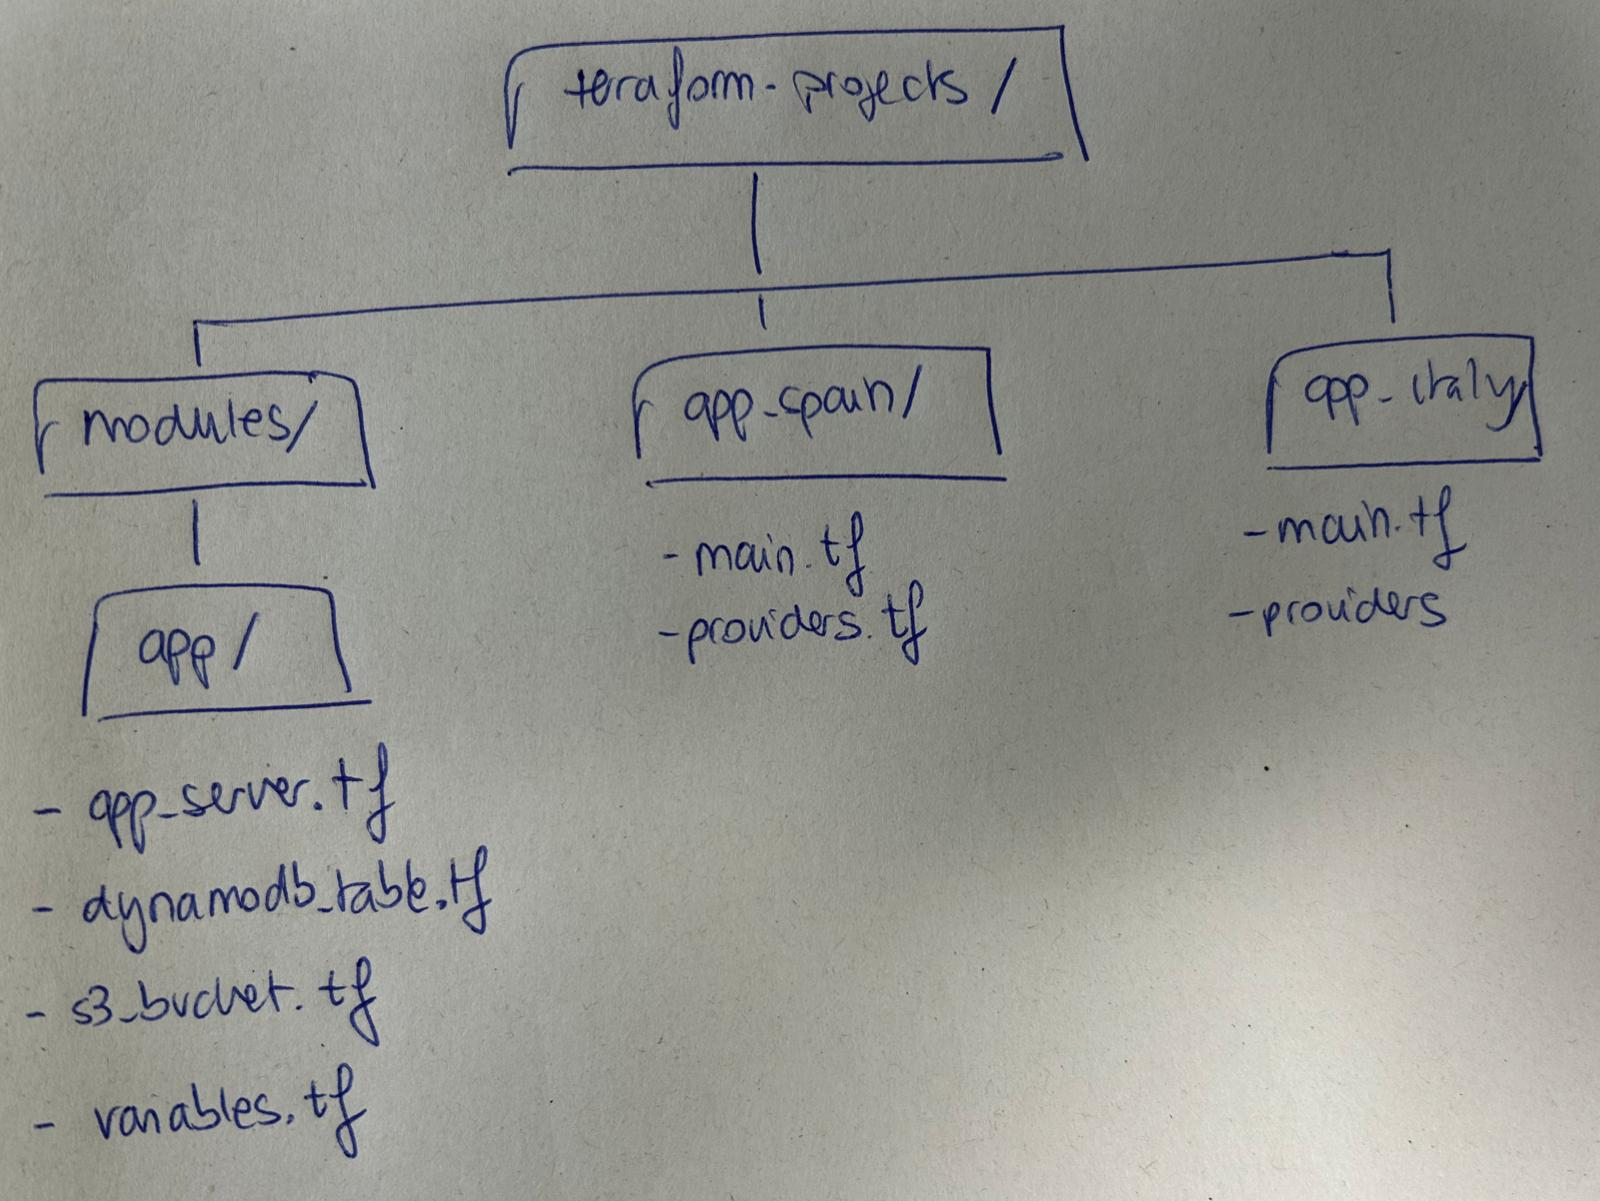
\includegraphics[width=\textwidth]{pictures/pic13.jpeg}
    \centering
\end{figure}

\begin{itemize}
    \item \verb|modules/app/|
\end{itemize}

\begin{codetemplate}{terrafom-projects/modules/app/app\_server.tf}
\begin{verbatim}
resource "aws_instance" "app_server" {
    ami           = var.ami
    instance_type = "t2.medium" # Hardcoded value
    tags          = {
        Name = "${var.app_region}-app-server"
    }
    
    depends_on = [ aws_dynamodb_table.payroll_db,
                   aws_s3_bucket.payroll_data   
                 ]
}
\end{verbatim}
\end{codetemplate}

\begin{codetemplate}{terrafom-projects/modules/app/s3\_bucket.tf}
\begin{verbatim}
resource "aws_s3_bucket" "payroll_data" {
    bucket = "${var.app_region}-${var.bucket}"
}
\end{verbatim}
\end{codetemplate}
\begin{codetemplate}{terrafom-projects/modules/app/dynamo\_table.tf}
\begin{verbatim}
resource "aws_dynamodb_table" "payroll_db" {
    name         = "user_data"        # Hardcoded value
    billing_mode = "PAY_PER_REQUEST"  # Hardcoded value
    hash_key     = "EmployeeID"       # Hardcoded value

    attribute {
        name = "EmployeeID"
        type = "N"
    }
}
\end{verbatim}
\end{codetemplate}

\begin{codetemplate}{terrafom-projects/modules/app/variables.tf}
\begin{verbatim}
variable "app_region" {
    type = string
}

variable "bucket" {
    type    = string
    default = "flexit-payroll-apha-ffasdf"
}

variable "ami" {
    type = string
}
\end{verbatim}
\end{codetemplate}

\begin{blocktemplateIII}{WARNING}
There are variables hardcoded because we dont want them to be changed from the root module
\end{blocktemplateIII}

\newpage
\begin{itemize}
    \item \verb|app_spain/:| root module
\end{itemize}
\begin{codetemplate}{terraform-projects/app\_spain/main.tf}
\begin{verbatim}
module "app_spain" {
    source     = "../modules/app"
    app_region = "us-east-1"
    ami        = "..."
}
\end{verbatim}
\end{codetemplate}

\begin{itemize}
    \item \verb|app_italy/:| root module
\end{itemize}
\begin{codetemplate}{terraform-projects/app\_italy/main.tf}
\begin{verbatim}
module "app_spain" {
    source     = "../modules/app"
    app_region = "us-east-2"
    ami        = "..."
}
\end{verbatim}
\end{codetemplate}

Modules are comparable to libraries or packages that are used in most programming languages, or comparable to roles in ansible.

Benefits:
\begin{itemize}
    \item Simpler configuration ocmpared to single configuration file with hundreds to thousands of lines.
    \item Our root module now it is very short and easy to understand and manage.
    \item Using a pre-configured module that has been tested and validated also decreases PBCAKs.
    \item Enables code reusability.
    \item Fix some variables of the configuration, to ensure they are not modified by the root module.
\end{itemize}

\subsection{Using Modules from Terraform Registry}

So far, we know that Terraform Registry is used to provide "providers", but it also used as a public repository that stores modules. The modules ono the Terraform Registry are sorted based on the provider for which they are created. They can be categorized into 2 types:
\begin{itemize}
    \item \textbf{Verified Modules:} tested and mantainer by HashiCorp.
    \item \textbf{Community Modules:} published by users on the community but not validated by HashiCorp.
\end{itemize} 

In some cases, the modules can contain several sub-modules that can be used for different use cases.

To use a remote module:

\begin{codetemplate}{main.tf}
\begin{verbatim}
module "security_group_ssh" {
    source     = "check/in/the/documentation"
    version    = 
    vpc_id     =
    name       = 
    ...
}
\end{verbatim}
\end{codetemplate}

\begin{blocktemplateII}{Note}
It is a good idea to specify the version of the module, if you don't specify the version, it will always download the latest version available of this module on the registry.
\end{blocktemplateII}

To just download the needed remote modules from registries:

\begin{codetemplate}{}
\begin{verbatim}
$ tf get
\end{verbatim}
\end{codetemplate}

\section{Terraform Functions}

\subsection{Already Learned Terraform Functions}

We have already used a few Terraform functions throughout this course:
\begin{itemize}
    \item \verb|file()|: to read data from a file.
    \item \verb|length()|: to determine the number of elements of a given list or map.
    \item \verb|toset()|: to convert a list into a set.
\end{itemize}

Terraform provides an interactive console that can be used for testing functions as well as interpolations. To get into this interactive console, we need to use the command:
\begin{codetemplate}{}
\begin{verbatim}
$ tf console
\end{verbatim}
\end{codetemplate}

The interactive console loads the state associated with the configuration directory by default allowing us to load any values that is currently stored on it. It also loads variables that are stored within configuration files.

Usage examples inside the console:

\begin{codetemplate}{tf console}
\begin{verbatim}
> file("/root/terraform-projects/main.tf")
> len(var.region)
\end{verbatim}
\end{codetemplate}

\subsection{Basic New Terraform Functions}
We can categorize functions in the following groups:
\begin{itemize}
    \item Numeric Functions
    \item String Functions
    \item Collection Functions
    \item Type Conversion Functions
\end{itemize}

\subsubsection{Numeric Functions}
To operate and manipulate numbers:
\begin{itemize}
    \item \verb+max(-1, 2, -10, 200)+ or \verb+max(var.my_list)+
    \item \verb+min(-1, 2, -10, 200)+ or \verb+min(var.my_list)+
    \item \verb|ceil(10.3):| to ceil a number.
    \item \verb|floor(10.3):| to ceil a number.
    \item ...
\end{itemize}

\subsubsection{String Functions}
To transform or manipulate strings:
\begin{itemize}
    \item \verb+split(" ", "Hola que ase")+: separate a string in a list of strings making use of the separator.
    \item \verb+lower(string)+
    \item \verb+upper(string)+
    \item \verb|title(string):| camel case.
    \item \verb|substr(string, offset, length)|: get the substring between the positions "offset" and "offset + length".
    \item \verb|join(",", ["hola", "que", "ase"])|: gather all the elements of a list in one single string.
    \item ...
\end{itemize}

\subsection{Collection Functions (lists and sets)}
\begin{itemize}
    \item \verb|lenght(collection)|
    \item \verb|index(collection, "element_value")|: to find the index of a matching element.
    \item \verb|element(collection, index):| to retrieve an element in a collection located at a specific index.
    \item \verb|contains(collection, "string to check"):| to check if an element is inside a list or not.
    \item ...
\end{itemize}

\subsection{Map Functions}
\begin{itemize}
    \item \verb|keys(map)|: to get the keys of a map into a list.
    \item \verb|values(map)|: to get the keys of a map into a list.
    \item \verb|lookup(map, "key")|: lookup the value for specific key, if it is not on the map, return an error.
    \item \verb|lookup(map, "key","default_return")|: if it is not on the map, return "\verb|default_return|"
    \item ...
\end{itemize}

\subsection{Usage example}
\begin{codetemplate}{variables.tf}
\begin{verbatim}
variable "cloud_users" {
    type = string
    default = "andrew:ken:faraz:mutsumi:peter:steve:braja"
}
\end{verbatim}
\end{codetemplate}
\begin{codetemplate}{main.tf}
\begin{verbatim}
resource "aws_iam_user" "cloud" {
    name = split(":", var.cloud_users)[count.index]
    count = length(split(":", var.cloud_users))
}
\end{verbatim}
\end{codetemplate}

\subsection{Operators}

Examples of automatic operations:
\begin{itemize}
    \item \verb|1 + 2|, \verb|1 - 2|.
    \item \verb|3 * 4|, \verb|1 / 2|.
    \item \verb|==|: equal operator returning a boolean.
    \item \verb|!=|: not equal operator returning a boolean.
    \item \verb|1 < 2, 1 > 2, 1 >= 2, 1 <= 2|: returning booleans.
    \item \verb|&&|: local "and" operation returning a boolean.
    \item \verb+||+: local "or" operation returning a boolean.
    \item \verb|!|: not operator before an other operator.
    \item ...
\end{itemize}

\subsection{Conditionals}

\begin{codetemplate}{}
\begin{verbatim}
condition ? true_val : false_val
\end{verbatim}
\end{codetemplate}

For example:
\begin{codetemplate}{main.tf}
\begin{verbatim}
resource "aws_instance" "mario_servers" {
    ami           = var.ami
    instance_type = var.name == "tiny" ? "t2.nano" : "t2.2xlarge"
    
    tags = {
        Name = var.name
    }
}      
\end{verbatim}
\end{codetemplate}

\section{Workspaces}

Erlier on this documentation, we learned about state and its use when running Terraform operatins. Wheter stored locally or in remote backend such as S3 or another Terraform Provider option. And, as we know, state is essential in mapping the real-world infrastructure allowing Terraform to model what changes it needs to apply based on the configuration defined in the state files. 

All the \verb|terraform.tfstate| files we have seen so far have one-to-one mapping between the configuration directory and the \verb|.tfstate| file. This means that we have one \verb|terraform.tfstate| file per configuration directory.

Imagine the example that we have 2 environments, PRO and PRE and we want to deploy the same object, just changing the ami. So far, the only option we know is using modules and two different directories for each environment. However, the goal of using Terraform or any IaC tool for that matter is to eliminate repeatable steps and efficiently make use of existing code. For that purpose, Terraform offer a feature that allows configuration files within a directory to be reused multiple times for different use cases, called \textbf{workspaces}.

With \textbf{workspaces} we can use the same configuration directory to create multiple infrastructure environments; such as PRO, PRE, TST, QA, etc.

To create a \textbf{workspace}:

\begin{codetemplate}{}
\begin{verbatim}
$ tf workspace new <workspace_name>
\end{verbatim}
\end{codetemplate}

\begin{blocktemplate}{Note}
Once a \textbf{workspace} is created, Terraform will immediately switch to it as well (not as git).
\end{blocktemplate}

To list the \textbf{workspaces} that have been created:
\begin{codetemplate}{}
\begin{verbatim}
$ tf workspace list
\end{verbatim}
\end{codetemplate}

\begin{blocktemplateII}{Note}
\textbf{default} workspace is always created when you init a Terraform project, but it is hardly recommended to use \textbf{custom workspaces} for large terraform projects.
\end{blocktemplateII}

To switch to an specific \textbf{workspaces} that have been already created:
\begin{codetemplate}{}
\begin{verbatim}
$ tf workspace select <workspace_name>
\end{verbatim}
\end{codetemplate}

So, in order to use different configurations for each \textbf{workspace} we will need to remove all the \textbf{hardcoded} values from \verb|main.tf| and put them all in \verb|variables.tf| file. For example:

\begin{codetemplate}{variables.tf}
\begin{verbatim}
variable region {
    type    = string
    default = "ca-central-1" 
}

variable instance_type {
    type    = string
    default = "t2.micro"
}

variable ami {
    type    = map
    default = {
        "PRO" = "ami-fkdapsñfkasñdj"
        "PRE" = "ami-0f80983409820p"
    }
}
\end{verbatim}
\end{codetemplate}

\begin{codetemplate}{main.tf}
\begin{verbatim}
resource "aws_instance" "PRO" {
    ami = lookup(var.ami, terraform.workspace)
    instance_type = var.instance_type
    tags          = {
        Name = terraform.workspace
    }
}
\end{verbatim}
\end{codetemplate}

Then, when we run \verb|tf apply| it will generate 2 different \verb|terraform.tfstate| files, one for each \textbf{workspace}, stored in a different directory:
\begin{codetemplate}{}
\begin{verbatim}
/path/to/terraform-project/terraform.tfstate.d/
\end{verbatim}
\end{codetemplate}

\end{document}